\documentclass[10pt,journal,compsoc]{IEEEtran}
% \UseRawInputEncoding
\usepackage{enumerate}
\usepackage{cite}
\usepackage{amsmath}
\interdisplaylinepenalty=2500
\usepackage{algorithm}
\usepackage{algorithmic}
\usepackage{graphicx}
\usepackage{multirow}
\usepackage{subfigure}
\usepackage{amssymb}
\usepackage[normalem]{ulem}
\usepackage{color}
\usepackage{amsmath}
\usepackage{array}
\usepackage{booktabs}
\hyphenation{op-tical net-works semi-conduc-tor}
\newcommand{\rmnum}[1]{\expandafter{\romannumeral #1\relax}}

\begin{document}

\title{Adaptive Metamorphic Testing: An approach to Improve the Fault Detection Efficiency of Metamorphic Testing}


\author{Chang-ai~Sun,~\IEEEmembership{Senior Member,~IEEE,}
        Hepeng~Dai,
        Huai Liu,~\IEEEmembership{Member,~IEEE,}
        and~Tsong Yueh~Chen,~\IEEEmembership{Member,~IEEE,}
\thanks{C.-A. Sun, and H. Dai are with the School of Computer and Communication Engineering, University of Science and Technology Beijing, Beijing 100083, China. E-mail: casun@ustb.edu.cn.}% <-this % stops a space
\thanks{H. Liu is with the College of Engineering and Science, Victoria University, Melbourne VIC 8001, Australia. E-mail: Huai.Liu@vu.edu.au.}
\thanks{T.Y. Chen is with the Department of Computer Science and Software Engineering, Swinburne University of Technology, Hawthorn VIC 3122, Australia. Email: tychen@swin.edu.au.}
}


\markboth{IEEE TRANSACTIONS ON SOFTWARE ENGINEERING,~submitted}%
{}


\IEEEtitleabstractindextext{
\begin{abstract}
  Metamorphic testing (MT) is a promising technique to alleviate the oracle problem, which first defines metamorphic relations (MRs) that are then used to generate new test cases (i.e. follow-up test cases) from the original test cases (i.e. source test cases), and verify the results of source and follow-up test cases. Many efforts have been reported to improve MT's efficiency by either generating better MRs that are more likely to be violated or selecting different test case selection strategies to generate source test cases. Unlike these efforts, we investigate how to improve the efficiency of MT in terms of test executions. Furthermore, traditional MT techniques often employ the random testing strategy (RT) to select source test cases for execution, which could be inefficient because the feedback information during the testing process is not leveraged. Consequently, we propose an adaptive metamorphic testing (AMT) technique to improve the efficiency of MT through controlling the execution process of MT. In the process of testing, AMT can quickly find source test cases and MRs with fault detected ability based on historical information of testing.  We conducted an empirical study to evaluate the efficiency of the proposed technique with four laboratory programs, a GNU program, and an Alibaba program. Empirical results show that AMT outperforms traditional MT in terms of fault-detecting efficiency.
\end{abstract}

\begin{IEEEkeywords}
metamorphic testing, control test process, feedback, random testing, adaptive random testing, partition testing, adaptive partition testing
\end{IEEEkeywords}}

\maketitle

\IEEEdisplaynontitleabstractindextext


\IEEEpeerreviewmaketitle


\section{Introduction}
\label{sec:introduction}

\IEEEPARstart{T}{est} result verification is an essential step of software testing. A test oracle \cite{weyuker1982testing} is a mechanism that can exactly decide whether the output produced by a programs is correct. However, there are situations where it is difficult to decide whether the result of the software under test (SUT) agrees with the expected result. This situation is known as oracle problem \cite{barr2015oracle, patel2018mapping}. In order to alleviate the oracle problem, several techniques have been proposed, such as N-version testing \cite{brilliant1990performance}, metamorphic testing (MT) \cite{chen1998metamorphic, chen2018metamorphic}, assertions \cite{sim2014eliminating}, and machine learning \cite{chan2009pat}. Among of them, MT obtains metamorphic relations (MRs) according to the properties of SUT. Then, MRs are used to generate new test cases called follow-up test cases from original test cases known as source test cases. Next, both source and follow-up test cases are executed and their result are verified against the corresponding MRs. MT checks whether a relevant MR holds among multiple executions. If an MR does not hold,then it can be concluded that the software system is faulty.

MT has been drawing increasing attention in the software testing community \cite{segura2016survey, chen2018metamorphic}, since this technique not only alleviates the oracle problem but also generates new test cases from existing test cases. The technique has been successfully applied in a number of application domains and paradigms, including healthcare \cite{murphy2011effective}, bioinformatics \cite{chen2009innovative}, air traffic control \cite{hui2013metamorphic}, the web service \cite{zhou2012automated}, the RESTful web APIs \cite{segura2018metamorphic}, and testing of AI systems \cite{tian2018deeptest, marijan2019challenges,zhang2020machine}. Observations from the existing evaluations indicate that MT is a new and promising strategy that complements the existing testing approaches \cite{Sun2019METRIC}.

There are two broad categories of methods to improve the effectiveness of MT: source test cases generating and MRs identifying. The former employs different test case selection strategies to generate source test cases for MT \cite{chen2004metamorphic, barus2016impact}. The latter creates MRs by combining existing relations, or by generating them automatically \cite{chen2004case, cao2013correlation, sun2011metamorphic, chen2016metric, xie2016looking}.

The fault-detecting effectiveness of MT relies on the quality of MRs and the source test cases. 
Chen et al. \cite{chen2004metamorphic} initially suggested all available MRs should be used as part of the test strategy. In the context of the resources for software development are always limited, 
Chen et al. \cite{chen2004case} proposed ``good'' MRs should be those that can make the multiple executions of the program as different as possible. Furthermore, they concluded that good MRs should be preferably selected with regard to the algorithm
under test following a white-box approach. 
However, this was later disputed by Mayer and Guderlei \cite{mayer2006empirical}, who studied six subject programs for matrix determinant computation with seeded faults. They concluded that metamorphic relations in the form of equalities or linear equations as well as those close to the implementation strategy have limited effectiveness. Conversely, they reported that good metamorphic relations are usually strongly inspired by the semantics of the program under test.
Asrafi et al. \cite{asrafi2011testing} concluded that the higher the combined code coverage of the source and follow-up test cases, the more different are the executions, and the more effective is the MR through a case study. 
The above three methods discuss the properties of ``good'' MRs from the point of view of the black-box and the white-box.
On the other hand, Just et al. \cite{Just2010Automating} assessed the applicability of metamorphic testing for system and integration testing in the context of an image encoder, and concluded that the MRs derived from the components of a system are usually better at detecting faults than those MRs derived from the whole system. To select ``good'' MRs, all of these methods require test cases to be executed before testing SUT. Without doubt, testing overhead is increased.

As for selection source test cases, 57\% of existing studies employed random testing (RT) to select test cases, and 34\% of existing studies used existing test suites according to a survey report by Segura et al. \cite{segura2016survey}. RT randomly selects test cases from input domain (which refers to the set of all possible inputs of SUT). Although RT is simple to implement, RT does not make use of any execution information about SUT or the test history. Thus, traditional MT may be ineffectiveness in some situations. The existing test suite may not adequately test the new version SUT. Because of the above limitations, Barus et al. \cite{barus2016impact} employed adaptive random testing (ART) \cite{chen2004adaptive} that is a class of testing method aimed to improve the performance of RT by increasing the diversity across a program's input domain of the test cases executed to generate source test cases for MT. However, the characteristics of ART itself (such as high time consumption, most algorithms only apply to numerical programs) will increase the time consumption of MT. 

In previous and existing work, it is difficult for practitioners to choose the MRs based on the existing work or need to consume a lot of resources to choose those ``good'' MRs. On the other hand, researchers have mainly focused on the impact of MRs, with the impact of source test cases on MT’s fault-detection effectiveness having somehow been neglected. In other words, investigation of the impact of
source test cases on MR (and MT) effectiveness is an area yet to be explored \cite{chen2018metamorphic}. Futhermore, researchers investigated the effectiveness of MT by either choosing different MRs alone, or choosing different test case selection strategies to generate source test cases alone. 

Different from the previous methods, this paper proposed an innovative method that makes use of feedback information to select both source test case and corresponding MR based on software cybernetics \cite{cangussu2007software, yang2017modern}, aiming to maximize the fault-detection effectiveness of MT.

In this study, we investigate how to make use of feedback information in the previous tests to control the execution process of MT in terms of both selecting source test cases and MRs, and proposed adaptive metamorphic testing method (AMT). AMT is built on top of three insights: \rmnum{1}) source test cases is one of factors that effects the fault-detecting efficiency of MT. However, random testing is commonly used to generate source test cases, and only a little researches related to use appropriate test cases selection strategies to generate source test cases \cite{segura2016survey}; \rmnum{2}) most of existing work help testers create MRs, aiming to improve the fault-detection efficiency of MT, while there seems to be no investigation to study how to choose an MR based on the generated set of MRs; \rmnum{3}) an appropriate test cases selection strategy can generate ``better" test cases (i.e. those test cases have a higher probability to detect a fault). In MT, if source test cases cannot detect a fault, and follow-up test case generated by an MR detect a fault, we still can conclude that this execution detect a fault. Therefore, based on a selected source test case, choosing a ``better" MR can improve the fault-detection efficiency.

In short, AMT collects feedback information during the test, and makes use of those information to select source test case and MRs.
As a result, a process-feedback metamorphic testing framework is proposed to improve the fault-detecting efficiency of MT. An empirical study was conducted to evaluate the efficiency of the proposed technique. Main contributions made in this paper are the following:

\begin{enumerate}[1]
  \item
  From a new perspective, we proposed a adaptive metamorphic testing method. This includes a general framework (AMT) that indicates how to make use of history testing information to select next source test case and dynamically select MR.
  \item
  We particular developed two algorithms (MAPT* and RAPT*) to select source test cases, and two algorithms (PBMR and RMRS) to select MRs for MT. Then the test case selection algorithms and MR selection algorithms were combined to obtain four AMT strategies: \rmnum{1}) MR-AMT and RR-AMT (MAPT* selects test cases and RMRS selects MRs, and RAPT* selects test cases and RMRS selects MRs, respectively), which first select a partition according to the test profile, and randomly select a test case from the selected partition and randomly selects a MR from the set of MRs whose source test cases belong to selected partition, then update test profile according to the result of test execution; \rmnum{2}) MP-AMT and RP-AMT (MAPT* selects test cases and PBMR selects MRs, and RAPT* selects test cases and PBMRs selects MRs, respectively) which first select a partition according to the test profile, and randomly select a test case from the selected partition and selects a MR from the set of MRs whose source test cases belong to selected partition according to PBMR algorithms, then update test profile according to the result of test execution.
  \item
  We evaluated the performance of AMT through a series of empirical studies on 6 programs, including four laboratory programs, GNU \texttt{grep}, and Alibaba \texttt{FastJson}. These studies show that AMT has significantly higher fault-detection efficiency than traditional MT that randomly selects source test cases and MRs.

\end{enumerate}


The rest of this paper is organized as follows.
Section \ref{sec:background} introduces the underlying concepts for MT, APT and CPM.
Section \ref{sec:amt} presents the AMT framework, the strategies of test case selection, and the strategies of MRs selection.
Section \ref{sec:empiricalStudy} describes an empirical study where the proposed AMT is used to test four laboratory programs, a Gun program, and an Alibaba program, the results of which are summarized in Section \ref{sec:results}.
Section \ref{sec:relatedwork} discusses related work and Section \ref{sec:conclusion} concludes the paper.

\section{Background}
\label{sec:background}

In this section, we present some of the underlying concepts for MT, and APT.

\subsection{Metamorphic Testing (MT)}

\label{section:mt}

MT is a novel technique to alleviate the oracle problem: Instead of applying an oracle, MT uses a set of MRs (corresponding to some specific properties of the SUT) to verify the test results \cite{chen1998metamorphic}. MT is normally conducted according to the following steps:

\begin{description}
  \item [Step1.]
  Identify an MR from the specification of the SUT.
  \item [Step2.]
  Generate the source test case $stc$ using the traditional test cases generation techniques.
  \item [Step3.]
  Derive the follow-up test case $ftc$ from the $stc$ based on the MR.
  \item [Step3.]
  execute $stc$ and $ftc$ and get their outputs $O_s$ and $O_f$.
  \item [Step4.]
  Verify $stc$, $ftc$, $O_s$, and $O_f$ against the MR: If the MR does not hold, a fault is said to be detected.
\end{description}
The above steps could be repeated for a set of MRs.

Let us use a simple example to illustrate how MT works. For instance, consider a program $P(G, a, b)$ purportedly calculating the length of the shortest path between nodes $a$ and $b$ in an undirected graph $G$. When G is nontrivial, the program is difficult to test because no oracle can be practically applied. Nevertheless, we can perform MT. Let $(G_1, a_1, b_1)$ and $(G_2, a_2, b_2)$ be two inputs, where $G_2$ is a permutation of $G_1$ (that is, $G_2$ and $G_1$ are isomorphic), and $(a_1, b_1)$ in $G_1$ correspond to $(a_2, b_2)$ in $G_2$. Then an MR can be identified as follows: $P(G_1, a_1, b_1) = P(G_2, a_2, b_2)$. A metamorphic
test using this MR will run $P$ twice, namely, a source execution on the source test case $(G_1, a_1, b_1)$ and a follow-up execution on the follow-up test case $(G_2, a_2, b_2)$.

\subsection{Category Partition Method (CPM)}
\label{sec:cpm}

Category partition method (CPM) is widely used specification-based testing technique \cite{ostrand1988category}. It helps software testers create test cases by refining the functional specification of a program into test specifications. The method consists of the following steps.

\begin{description}
  \item [Step1.]
  Decompose the functional specification into functional units that can be tested independently, then Identify the parameters (the explicit inputs to a functional unit) and environment conditions (the state of the system at the time of execution) that are known as \emph{categories}.
  \item [Step2.]
  Partition each \emph{category} into \emph{choices}, which include all the different kinds of values that are possible for that \emph{category}.
  \item [Step3.]
  Determine the constraints among the \emph{choices} of different \emph{categories}, and Write the test specification (which is a list of categories, choices, and constraints in a predefined format) using the test specification language TSL.
  \item [Step4.]
  Use a generator to produce \emph{test frames} from the test specification. Each generated \emph{test frame} is a set of choices. Then, create a test case by selecting a single element from each \emph{choice} in each generated \emph{test frame}.
\end{description}

In this study, we made use of CPM to create test cases. During the process of testing, the choice information can be used as the basis for choosing the MRs. The proposed AMT selects both source test cases and corresponding MRs by making use of information which is collected during the test process that means, we need to establish a connection between the source test cases and MRs. The connection provides a guideline for us to obtain the set of candidate MRs according to a source test case or select a source test case for an MR.

\subsection{Adaptive Partition Testing (APT)}
\label{sec:apt}

Based on software cybernetics, which aims to explore the interplay between software engineering and control theory, Sun \cite{sun2018adaptive} propose a new testing approach, adaptive partition testing (APT), where test cases are randomly selected from some partition $c_i$ whose probability $p_i$ of being selected is adaptively adjusted along the testing process. The main concept of APT is to increase the selection probabilities of the partitions which have higher defect detected rates. If a defect is detected by some test cases from partition $c_i$, then $c_i$ is considered to have a higher defect detected rate and an increment is added to $p_i$; Otherwise, $p_i$ is decreased.

Furthermore, they particularly develop two algorithms, Markov-chain based adaptive partition testing (MAPT) and
reward-punishment based adaptive partition testing (RAPT), to implement the proposed approach. MAPT and RAPT algorithms assume that testers can obtain test oracles, therefore, MAPT and RAPT are difficult to apply when there are no test oracles or it is
difficult to obtain the test oracles. 

\subsubsection{Markov-Chain Based Adaptive Partition Testing (MAPT)}
\label{sec:mapt}

According to the concept of Markov chain, given two states $i$ and $j$, the probability of transitioning from $i$ to $j$ is represented by $p_{i,j} = Pr\{j|i\}$. For $i = 1, 2, \ldots, m$ we can then construct a Markov matrix as follows:

\begin{equation}
\label{eq:matrix}
\mathcal{P} =
\begin{pmatrix}{}
  p_{1,1} & p_{1,2} & \cdots & p_{1,m} \\
  p_{2,1} & p_{2,2} & \cdots & p_{2,m} \\
  \vdots  & \vdots  & \ddots & \vdots  \\
  p_{m,1} & p_{m,2} & \cdots & p_{m,m}
\end{pmatrix}
\end{equation}

In MAPT, each partition is considered as a state in the Markov matrix. If a partition $s_i$ is selected for conducting a
test, the probability of selecting $s_i$ for conducting the next test will be $p_{i,j}$. MAPT will adaptively adjust the value of
each $p_{i,j}$ according to the testing result. The algorithm of MAPT is available in \cite{sun2018adaptive}.

\subsubsection{reward-punishment based adaptive partition testing (RAPT)}
\label{sec:rapt}

Based on the reward and punishment mechanism, RAPT attempts to be quicker at selecting the fault-revealing test cases. Two parameters $Rew_i$ and $Pun_i$ are used in RAPT to determine to what extent a partition $c_i$ can be rewarded and punished, respectively. If a test case in $c_i$ reveals a fault, $Rew_i$ will be incremented by 1 and $Pun_i$ will become 0, and test cases will be repeatedly selected from $c_i$ until a non-fault-revealing test case is selected from $c_i$. If a test case selected from $c_i$ does not reveal a fault, $Rew_i$ will become 0 and $Pun_i$ will be incremented by 1. If $Pun_i$ reaches a preset bound value $Bou_i$, $c_i$ will be regarded to have a very low failure rate, and its corresponding $p_i$ will become 0. The algorithm of RAPT is available in \cite{sun2018adaptive}.

\begin{figure*}[htb]
  \centering
  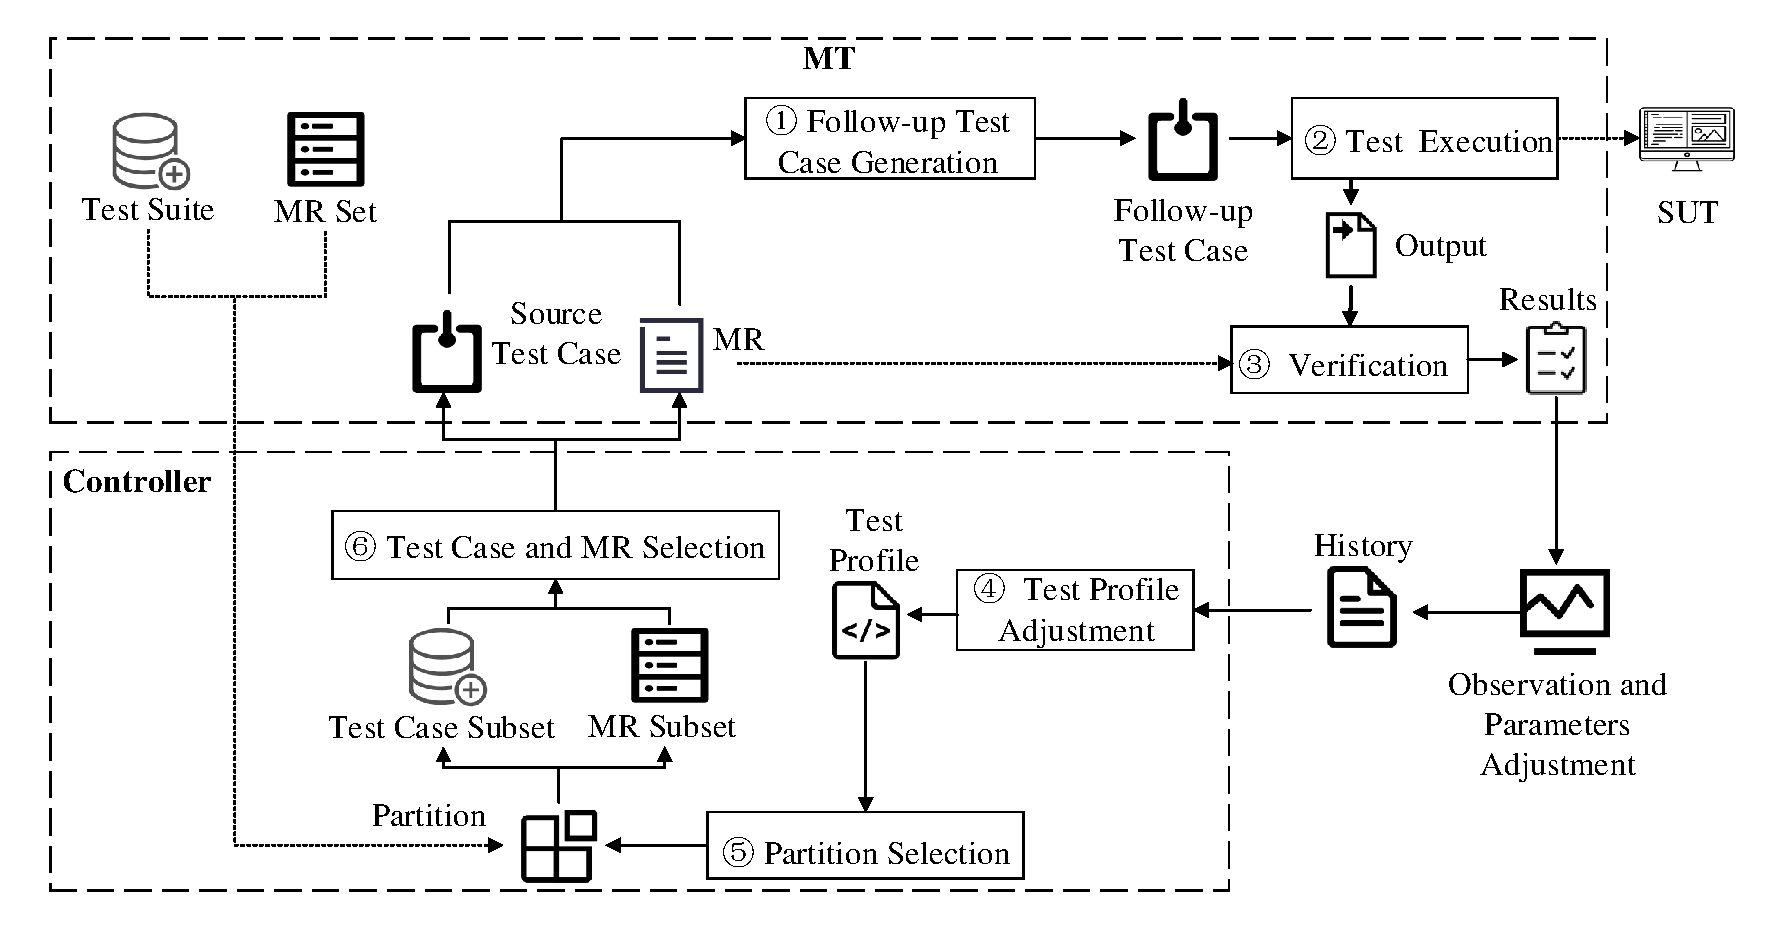
\includegraphics[width = 0.8\textwidth]{fig//framework}
  \caption{The Framework of AMT}
  \label{fig:framework}
\end{figure*}

\section{Adaptive Metamorphic Testing}
\label{sec:amt}
In this section, we present the motavation of this paper, describe a framework for process-feedback MT, and argorithms about selection source test cases and MRs.

\subsection{Motivation}
\label{sec:motavation}

Since MT was first published, a considerable number of studies have been reported from various aspects \cite{segura2016survey}. To improve the efficiency of MT, most of studies have paid their attention to identify the better MRs, which are more likely to be violated. For the  efficiency of MRs, several factors such as the difference between the source and follow-up test cases \cite{chen2004case, cao2013correlation} and the the detecting-faults capacity of MRs compared to existing test oracles \cite{liu2014effectively}, have been investigated.

Since the follow-up test cases are generated based on source test cases and MRs, in addition to the so-called good MRs, source test cases also have an impact on the efficiency of MT. However, 57\% of existing studies employed RT to select test cases, and 34\% of existing studies used existing test suites according to a survey report by Segura et al. \cite{segura2016survey}. In this study, we investigate the strategies of selection test cases and MRs, and its impacts on the fault-detecting efficiency of MT.

It has been pointed out that fault-detecting inputs tend to cluster into ``continuous regions'' \cite{ammann1988data, finelli1991nasa}, that is, the test cases in some partitions are more likely to detect faults than the test cases in other partitions. Inspired by the observation, AMT takes full advantage of feedback information to update the test profile, aiming at increasing the selection probabilities of partitions with larger failure rates. Accordingly, the MRs whose sources test cases belonging to the partitions with larger failure rates, are more likely to be selected and violated. Therefore, AMT is expected to detect faults more efficient than traditional MT.

\subsection{Framework}
\label{sec:framework}

Considering the principles of software cybernetics and the features of MT, we propose an adaptive metamorphic texting framework, as
illustrated in Figure \ref{fig:framework}. As shown in Figure \ref{fig:framework}, there is a feedback loop in the AMT framework, which constitutes the components of MT, the software under test, the database (history of testing data) and the testing strategy (controller), where the history of testing data is used to generate the next test case and MR. Besides, the history of testing data is used to improve the underlying testing strategy. The improvement may lead he partition with higher failure rate has greater probability of being selected and the partition with lower failure rate has a lower probability of being selected. Interactions between AMT components are depicted in the framework. We next discuss the individual framework components.

\begin{enumerate}[1]  
  \item
  \emph{Follow-up Test Case Generation}. The follow-up test case is derived from the selected source test case based on the selected MR.

  \item
  \emph{Test Execution}. The relevant AMT component receives the generated source test case and follow-up test case, and executes them on SUT.

  \item
  \emph{Verification}.  The output of source and follow-up test case are verified against the corresponding MR. MT checks whether the relevant MR holds among multiple executions. If the MR does not hold, then it can be concluded that the software system is
  faulty.
\end{enumerate}

The component of \emph{Observation and Parameters Adjustment} is responsible for providing information to the controller. Upon completion of each test, its pass or fail status is determined by verifying the results of source test case and follow-up test case against corresponding MR. The pass or fail status are collected, and this information is used to adjust the test profile and update the values of parameters (probability adjusting factor) in the test case and MR selection strategies.

The controller is responsible for guiding the selection of test case and MR. In this paper, our testing strategy is based on partition testing (PT), which refers to a class of testing techniques that classify the input domain into a number of partitions \cite{weyuker1991analyzing}. After constructing partitions, Testers need to initialize the test profile, a simple way of doing which would be the use of a uniform probability distribution $P_1 = p_2 = \ldots = p_k$, where $k$ denotes the number of partitions, and $p_i (i = 1, 2, \ldots , k)$ denotes the probability of selecting the $i^{th}$ partition. Besides, the tester needs to create a subset $R_i (i = 1, 2, \ldots, k)$ of MRs for each partition $s_i$ so that any test case belonging to partition $p_i$ can generate follow-up test case driven by any MR belonging to $R_i$. During the testing process, the controller consists of the following procedure:

\begin{enumerate}[4]
  \item
  \emph{Test Profile Adjustment}. The controller updates the test profile with the historical data, so that the partitions with higher failure rate has a higher selection probability.
\end{enumerate}
\begin{enumerate}[5]
  \item
  \emph{Partition Selection}. AMT randomly selects a partition according to the test profile.
\end{enumerate}
\begin{enumerate}[6]
  \item
  \emph{Test Case and MR Selection}.  The tester needs to create a subset $R_i (i = 1,2,\ldots,k)$ of MRs for each
  partition $s_i$ so that any test case belonging to partition $s_i$ can generate follow-up test case driven by any MR belonging to $R_i$. Once a partition is selected, a test case and MR can be selected based on the proposed test case and MR selection strategies, respectively.
\end{enumerate}

\subsection{Source Test Case Selection}
\label{sec:stcs}

The previous MAPT and RAPT algorithms assume that testers can obtain test oracles, therefore, MAPT and RAPT are difficult to apply when there are no test oracles or it is difficult to obtain the test oracles. In this paper, we proposed two test case selection strategies MAPT* and RAPT* based on the MAPT and RAPT to select test cases in the context of MT.

\subsubsection{MAPT*}
\label{sec:mapt*}
Suppose that source test case $tc$ and corresponding follow-up test case $tc'$ are belonging to partition $s_{s}$ and $s_f$, respectively. if their results vioate the related MR, $\forall i = 1, 2, \ldots, m$ and $s, f \ne i$, we update test profile using the following equations. When source test case and follow-up test case belong to same partition ($s = f$), we set
\begin{equation}
\label{eq:MAPTKillOneSameI}
p'_{s, i} =
\begin{cases}
p_{s, i} - \displaystyle\frac{\gamma \times p_{s, s}}{m - 1}  & \text{if } p_{s, i} > \displaystyle\frac{\gamma \times p_{s, s}}{m - 1}\\
p_{s, i}                                                      & \text{if } p_{s, i} \leq \displaystyle\frac{\gamma \times p_{s, s}}{m - 1}
\end{cases}
\end{equation}
and then,

\begin{equation}
\label{eq:MAPTKillOneSameS}
p'_{s, s} = 1 - \sum\limits_{i = 0, i \ne s}^{m}p'_{s, i}.
\end{equation}

Alternatively, if $s \ne f$, we set

\begin{equation}
\label{eq:MAPTKillOneNotSameSI}
p'_{s, i} =
\begin{cases}
p_{s, i} - \displaystyle\frac{\gamma \times p_{s, s}}{m - 1}& \text{if }p_{s, i} > \displaystyle\frac{\gamma \times p_{s, s}}{m - 1} \\
p_{s, i}                                                    & \text{if } p_{s, i} \leq \displaystyle\frac{\gamma \times p_{s, s}}{m - 1}
\end{cases}
\end{equation}

\begin{equation}
\label{eq:MAPTKillOneNotSameFI}
p'_{f, i} =
\begin{cases}
p_{f, i} - \displaystyle\frac{\gamma \times p_{f, f}}{m - 1}& \text{if }p_{f, i} > \displaystyle\frac{\gamma \times p_{f, f}}{m - 1} \\
p_{f, i}                                                    & \text{if } p_{f, i} \leq \displaystyle\frac{\gamma \times p_{f, f}}{m - 1}
\end{cases}
\end{equation}
and then,
\begin{equation}
\label{eq:MAPTKillOneNotSameSS}
p'_{s, s} = 1 - \sum\limits_{i = 0, i \ne f}^{m}p_{s, i}
\end{equation}

\begin{equation}
\label{eq:MAPTKillOneNotSameFF}
p'_{f, f} = 1 - \sum\limits_{i = 0, i \ne f}^{m}p_{f, i}
\end{equation}

When source test case and corresponding follow-up test case donot detect a fault, we employ the following equations to update test profile. If source test case and correspnding follow-up test case belong to same partition ($s = f$), we set

\begin{equation}
\label{eq:MAPTNotKillOneSameSI}
p'_{s, i} =
\begin{cases}
p_{s, i} + \displaystyle\frac{\tau \times p_{s, i}}{m - 1} & \text{if } p_{s, s} > \displaystyle\frac{\tau \times (1 - p_{s, s})}{m - 1} \\
p_{s, i}                                                   & \text{if } p_{s, s} \leq \displaystyle\frac{\tau \times (1 - p_{s, s})}{m - 1}
\end{cases}
\end{equation}
and then,
\begin{equation}
\label{eq:MAPTNotKillOneSameSS}
p'_{s, s} =
\begin{cases}
p_{s, s} - \displaystyle\frac{\tau \times (1 - p_{s, s})}{m - 1}  & \text{if } p_{s, s} > \displaystyle\frac{\tau \times (1 - p_{s, s})}{m - 1} \\
p_{s, s}                                                          & \text{if } p_{s, s} \leq \displaystyle\frac{\tau \times (1 - p_{s, s})}{m - 1}
\end{cases}
\end{equation}

Alternatively, if $s \ne f$, we set
\begin{equation}
\label{eq:MAPTNotKillOneNotSameSI}
p'_{s, i} =
\begin{cases}
p_{s, i} + \displaystyle\frac{\tau \times p_{s, s}}{m - 1} & \text{if } p_{s, s} > \displaystyle\frac{\tau \times (1 - p_{s, s})}{m - 1} \\
p_{s, i}                                                   & \text{if } p_{s, s} \leq \displaystyle\frac{\tau \times (1 - p_{s, s})}{m - 1}
\end{cases}
\end{equation}

\begin{equation}
\label{eq:MAPTNotKillOneNotSameSS}
p'_{s, s} =
\begin{cases}
p_{s, s} - \displaystyle\frac{\tau \times (1 - p_{s, s})}{m - 1} & \text{if } p_{s, s} > \displaystyle\frac{\tau \times (1 - p_{s, s})}{m - 1} \\
p_{s, s}                                                         & \text{if } p_{s, s} \leq \displaystyle\frac{\tau \times (1 - p_{s, s})}{m - 1}
\end{cases}
\end{equation}

\begin{equation}
\label{eq:MAPTNotKillOneNotSameFI}
p'_{f, i} =
\begin{cases}
p_{f, i} + \displaystyle\frac{\tau \times p_{f, f}}{m - 1} & \text{if } p_{f, f} > \displaystyle\frac{\tau \times (1 - p_{f, f})}{m - 1} \\
p_{f, i}                                                   & \text{if } p_{f, f} \leq \displaystyle\frac{\tau \times (1 - p_{f, f})}{m- 1}
\end{cases}
\end{equation}

\begin{equation}
\label{eq:MAPTNotKillOneNotSameFF}
p'_{f, f} =
\begin{cases}
p_{f, f} - \displaystyle\frac{\tau \times (1 - p_{f, f})}{m - 1} & \text{if } p_{f, f} > \displaystyle\frac{\tau \times (1 - p_{f, f})}{m - 1} \\
p_{f, f}                                                         & \text{if } p_{f, f} \leq \displaystyle\frac{\tau \times (1 - p_{f, f})}{m - 1}
\end{cases}
\end{equation}

\subsubsection{RAPT*}
\label{sec:rapt*}

When source test case and follow-up test case belong to same partition ($s = f$), we set,

\begin{equation}
\label{eq:RAPTKillOneSameI}
p'_i =
\begin{cases}
p_i - \displaystyle\frac{(1 + lnRe_{w_i}) \times \epsilon}{m - 1} & \text{if } p_i > \displaystyle\frac{(1 + lnRe_{w_i}) \times \epsilon}{m - 1} \\
0                                                                 & \text{if } p_i \leq \displaystyle\frac{(1 + lnRe_{w_i}) \times \epsilon}{m - 1}
\end{cases}
\end{equation}
and then we have
\begin{equation}
\label{eq:RAPTKillOneSameS}
p'_s = 1 - \sum\limits_{i = 0, i \ne s}^mp'_i
\end{equation}
Alternativelt, if $s \ne f$, we set
\begin{equation}
\label{eq:RAPTKillOneNotSameI}
p'_i =
\begin{cases}
p_i - \displaystyle\frac{(1 + lnRe_{w_i}) \times \epsilon}{m - 2} & \text{if } p_i > \displaystyle\frac{(1 + lnRe_{w_i}) \times \epsilon}{m - 2} \\
0                                                                 & \text{if } p_i \leq \displaystyle\frac{(1 + lnRe_{w_i}) \times \epsilon}{m - 2}
\end{cases}
\end{equation}
and then we have
\begin{equation}
\label{eq:RAPTKillOneNotSameS}
p'_s = p_s + \displaystyle\frac{1 - \sum\limits_{i = 0, i \ne s, i \ne f}^mp'_i - p_s - p_f}{2}
\end{equation}

\begin{equation}
\label{eq:RAPTKillOneNotSameF}
p'_f = p_f + \displaystyle\frac{1 - \sum\limits_{i = 0, i \ne s, i \ne f}^mp'_i - p_s - p_f}{2}
\end{equation}

When source test case and corresponding follow-up test case donot detect a fault, we employ the following equations to update test profile. If source test case and correspnding follow-up test case belong to same partition ($s = f$), we set
\begin{equation}
\label{eq:RAPTNotKillOneSameS}
p'_s =
\begin{cases}
p_s - \delta & \text{if } p_s > \delta \\
0            & \text{if } p_s \leq \delta \text{ or } Pun_i = Bou_i,
\end{cases}
\end{equation}
and then
\begin{equation}
\label{eq:RAPTNotKillOneSameI}
p'_i =
\begin{cases}
p_i + \displaystyle\frac{\delta}{m - 1} & \text{if } p_s > \delta \\
p_i + \displaystyle\frac{p_s}{m - 1}            & \text{if } p_s \leq \delta \text{ or } Pun_i = Bou_i,
\end{cases}
\end{equation}

Alternatively, if $s \ne f$, we have
\begin{equation}
\label{eq:RAPTNotKillOneSameS}
p'_s =
\begin{cases}
p_s - \delta & \text{if } p_s > \delta \\
0            & \text{if } p_s \leq \delta \text{ or } Pun_i = Bou_i,
\end{cases}
\end{equation}

\begin{equation}
\label{eq:RAPTNotKillOneSameF}
p'_f =
\begin{cases}
p_f - \delta & \text{if } p_f > \delta \\
0            & \text{if } p_f \leq \delta \text{ or } Pun_i = Bou_i,
\end{cases}
\end{equation}
and then
\begin{equation}
\label{eq:RAPTNotKillOneSameI}
p'_i = p_i + \displaystyle\frac{(p_s - p'_s) + (p_f - p'_f)}{m - 2}
\end{equation}


In AMT, once a source test case is selected, the corresponding candidate MRs are available. We first proposed a simple strategy based on random mechanism to select an MR from the set of candidate MRs, then we proposed an innovative strategy to select an MR that can make the execution of follow-up test case as different as possible from the source test case.


\subsection{Dynamic MR Selection Strategies}
\label{sec:mrselection}

\subsubsection{Randomly MR-Selection Strategy (RMRS)}
\label{sec:rsmr}

RSMR randomly selects an from the set of candidate MRs, which is a straightforward method without considering extra information.

\subsubsection{Properties-Based strategy of MR selection (PBMR)}
\label{sec:pbmr}

The fault-detection efficiency of MT highly dependent on the specific MRs that are used, and selecting effective MRs is thus a critical step when applying MT. Chen et al. reported that good metamorphic relations are those that can make the execution of the source-test case as different as possible to its follow-up test case. Moreover, They defined the ``difference among execution" as any aspects of program runs (e.g., paths traversed).
Before presenting the properties-based strategy of MR selection (PBMR), we first introduce a new metric called category-partition-based metric (CP-distance) that measures the distance between the source test cases and corresponding follow-up test cases. CP-distance makes use of the concepts of categories and choices from the CPM method described in Section \ref{sec:cpm}. CP-distance have the capacity to reflect the difference among the source test cases and follow-up test cases, since the categories and choices are defined based on the software functionalities.

More formally, let us denote the set of categories by $A = \{A_1, A_2, \ldots, A_g\}$, where $g$ denotes the total number of categories. For each $A_i$, its choices are denotes by $P_i^{A_i} = \{p_1^{A_i},p_2^{A_i}, \ldots, p_h^{A_i}\}$, where $h$ denotes the number of choices for $A_i$. For input $x$, let us denote the corresponding non-empty subset by $A(x) = \{A_1^{x}, A_2^{x}, \ldots, A_q^{x}\}$, where $q$ refers to the number of categories associated with $x$. Since categories are distinct and their choices are disjoint, input $x$ in fact consists of values chosen from a non-empty subset of choices, denoted as $P(x) = \{p_1^{x}, p_2^{x}, \ldots, p_q^{x}\}$, where $p_i^x (i = 1, 2, \ldots, q)$ is the choice of the category $A_i^{x}$  for $x$.

For any two inputs $x$ and $y$, we define $DP(x,y)$ as the set that contains elements in either $P(x)$ or $P(y)$ but not both. That is,
$$DP(x,y) = (P(x) \cup P(y))\\ (P(x) \cap P(y)),$$ where ``n" is the set difference operator. Now, we define $$DA(x, y) = \{A_m|A_i if p_j^i \in DP(x, y)\}.$$ In other words, $DA(x, y)$ is the set of categories in which inputs $x$ and $y$ have different choices. Then, the distance measure between $x$ and $y$ is defined as $|DA(x, y)|$ (the size of $DA(x, y)$); that is, the number of categories that appear in either $x$ or $y$ but not both, or in which the choices in $x$ and $y$ differ.

obviously, a greater value of CP-distance representing more dissimilar execution. After selecting a source test case $stc_i$ and obtaining a set of candidate MRs $\mathcal{R} = \{r_1^{stc_i}, r_2^{stc_i}, \ldots, r_g^{stc_i}\}$ ($g$ is the number of MRs whose source test case could be $stc_i$), PBMR generate a set of candidate folow-up test cases $FC = \{ftc_{r_1^{stc_i}}, ftc_{r_2^{stc_i}}, \ldots, ftc_{r_g^{stc_i}}\}$ according to every MR belonged to $FC$. Then, the distance $CP_{i,h}$ ($h \in \{1,2, \ldots, g\}$) between $stc_i$ and each follow-up test case $ftc_{r_h^{stc_i}}$ is calculated. Finally, the MR $r_h^{stc_i}$ is selected as long as the following condition is hold:
$$CP_{i,h} = max\{CP_{i,1}, CP_{i,2}, \ldots, CP_{i,g}\}.$$

The details of PBMR is given in Algorithm \ref{alg:pbmr}.
\begin{algorithm}
\caption{PBMR}
\label{alg:pbmr}
    \begin{algorithmic}[1]
    \renewcommand{\algorithmicrequire}{\textbf{Input:}}
    \renewcommand{\algorithmicensure}{\textbf{Output:}}
    \renewcommand{\algorithmicendwhile}{\algorithmicend\_\algorithmicwhile}
    \renewcommand{\algorithmicendif}{\algorithmicend\_\algorithmicif}
    \REQUIRE $stc_i, \mathcal{R} = \{r_1^{stc_i}, r_2^{stc_i}, \ldots, r_g^{stc_i}\}, CParray = null$
    \ENSURE $CP_{max}$ ($max \in \{1, 2, \ldots, g\}$)
    \FOR {$h=1 \to h=g$}
    \STATE Generate the follow-up test case $ftc_h$ according to the $stc_i$ and $r_h^{stc_i}$
    \STATE Calculate the distance $CP_{i,h}$ between the $stc_i$ and $ftc_h$
    \STATE Add $CP_{i,h}$ to the list $CParray$
    \ENDFOR
    \STATE Calculate the maximal value $CP_{max}$ ($max \in \{1, 2, \ldots, g\}$) in the list $CParray$
    \end{algorithmic}
\end{algorithm}

\section{Empirical Study}
\label{sec:empiricalStudy}

We conducted a series of empirical studies to evaluate the performance of AMT.

\subsection{Research Questions}
\label{sec:rqs}
In our experiments, we focused on addressing the following two research questions:
\begin{description}
  \item [\textbf{RQ1}] \textbf{Could the proposed AMT strategy detect failures faster than MT?}

  Fault-detection efficiency is a key criterion for evaluating the performance of a testing technique. In our study, we chose four Laboratory programs, a GNU program, and an Alibaba program to evaluate the fault-detecting efficiency.

  \item [\textbf{RQ2}] \textbf{What is the actual test case and MR selection overhead when using the AMT technique?}

  We evaluate the test case and MR selection overhead of M-AMT and compare with traditional MT in detecting software faults.
\end{description}

\subsection{Object Programs}
\label{sec:programs}

In order to evaluate the fault-detection effectiveness of proposed methods in different scales, different implementation languages, and different fields, we chose to study three sets of object programs: four laboratorial programs that were developed according to corresponding specifications\footnote{The implementations have been made available at: https://github.com/phantomDai/subjects4tsc.git}, the regular expression processor component of the larger utility program \texttt{GNU grep}, and a Java library developed by Alibaba\footnote{This project is available at https://github.com/alibaba/fastjson}, which can be used to convert Java Objects into their JSON representation, and convert a JSON string to an equivalent Java object. Table \ref{table:objects} summarized the basic information of the object programs, giving the developer of object programs (\emph{Developer}), the name of object program (\emph{Program}), the size of the object program (\emph{LOC}), the number of total faults for each object program (\emph{Number of All Faults}), the number of used faults in each object program (\emph{Number of Used Faults}), test cases in the associated test pool (\emph{Size of test suite}), the number of identified MRs for each object program (\emph{Number of MRs}), and the number of partition for each object program (\emph{Number of Partitions}).

\begin{table*}[hbt]
  \caption{Six Programs as Experimental Objects}
  \label{table:objects}
  \centering
  \begin{tabular}{lllllllll} \toprule
  \multirow{2}{*}{Developer}&\multirow{2}{*}{Program}&\multirow{2}{*}{Language}&\multirow{2}{*}{LOC}&\multirow{2}{*}{All Faults}
  &\multirow{2}{*}{Used Faults} &Number of &Number of  &Number of  \\
  & & & &          &            &Test Cases&MRs        &Partitions\\ \midrule
                                &\texttt{CUBS}        &Java      &107     &187        &3    &368     &184        &8 \\
  \multirow{2}{*}{Laboratory}   &\texttt{ACMS}        &Java      &128     &210        &3    &284     &142        &4 \\
								&\texttt{ERS}         &Java      &117     &180        &1    &2260     &1130       &12 \\
								&\texttt{MOS}         &Java      &135     &215        &1    &7024     &3512       &9  \\ \midrule
  GNU                           &\texttt{grep}        &C         &10,068  &20         &8    &101,193 &12         &550 \\ \midrule
                                &\texttt{FastJson\_v31}    &Java      &125,192  &1          &1    &16,383  &17         &128 \\
  \multirow{2}{*}{Alibaba}      &\texttt{FastJson\_v36}    &Java      &134,440  &1          &1    &16,383  &17         &128 \\
                                &\texttt{FastJson\_v40}    &Java      &144,044  &1          &1    &16,383  &17         &128 \\
                                &\texttt{FastJson\_v48}    &Java      &149,544  &1          &1    &16,383  &17         &128 \\ \bottomrule
  \end{tabular}
\end{table*}

Based on four real-lift specifications, We developed four systems, which were implemented using Java programming language.
A detailed description of each laboratory program is given in the following.
\begin{enumerate}[1]
  \item
  \texttt{Expense Reimbursement System (ERS)} provides an interface through which customers can know how much they need to pay according to plans, month charge, calls, and data usage.
  \item
  \texttt{Aviation Consignment Management System (ACMS)} aims to help airline companies check the allowance (weight) of free baggage, and the cost of additional baggage. Based on the destination, flights are categorized as either domestic or international. For international flights, the baggage allowance is greater if the passenger is a student (30kg), otherwise it is 20kg. Each aircraft offers three cabins classes from  which to choose (economy, business, and first), with passengers in different classes having different allowances.
  \item
  \texttt{Expense Reimbursement System (ERS)} assists the sales Supervisor of a company with handling the following tasks: \rmnum{1}) Calculating the cost of the employee who use the cars based on their titles and the number of miles actually traveled; \rmnum{2}) accepting the requests of reimbursement that include airfare, hotel accommodation, food and cell-phone expenses of the employee.
  \item
  \texttt{Meal Ordering System (MOS)} helps catering provider to determine the quantity for every type of meal and other special
  requests (if any) that need to be prepared and loaded onto the aircraft served by this provider. For each flight, \texttt{MOS} generates a Meal Schedule Report (MSR), containing the number of various types of meals (first class, business class, economy class, vegetarian, child, crew member, and pilot) and the number of bundles of flowers.
\end{enumerate}

The used version of the \texttt{grep} programs is 2.5.1a \cite{grep}. This program searches one or more input files for lines containing a match to a specified pattern. By default, grep prints the matching lines. We chose \texttt{grep} for our study for several reasons:
\begin{enumerate}[1]
  \item
  \texttt{grep} program is wide used in Unix system, providing a opportunity to demonstrate the real world relevance of our techniques.
  \item
  \texttt{grep} program, and its input format, are of greater complexity than the the programs in the other test sets, but still manageable as a target for automated test case generation.
  \item
  \texttt{grep} program has been studied by several papers \cite{barus2014novel, barus2016impact, barus2016cost}, that means, we can obtain its faults, source test cases and MRs freely and conveniently.
\end{enumerate}

The inputs of the \texttt{grep} were categorize into three components: options, which consist of a list of commands to modify the searching process, pattern, which is the regular expression to be searched for, and files, which refers to the input files to be searched. The scope of functionality of this program is larger, which leads to construct test infrastructure to test all of functionality would have been impractical. Therefore, we restricted our focus to the regular expression analyzer of the \texttt{grep}.

\texttt{FastJson} is a Java library that can be used to convert Java Objects into their JSON representation (known as serialization). It can also be used to convert a JSON string to an equivalent Java object (known as deserialization
). We chose \texttt{FastJson} for our study for several reason:

\begin{enumerate}[1]
  \item
  \texttt{FastJson} is wide used in real-word projects, providing a opportunity to demonstrate the real world relevance of our techniques.
  \item
  \texttt{FastJson} is more complex than other programs, and it is a open source project, that is, we can obtain its faults freely and conveniently.
\end{enumerate}

The scope of functionality of this program is larger, which leads to construct test infrastructure to test all of functionality would have been impractical. Therefore, we restricted our focus to the deserialization of the \texttt{FastJson}. Two bigger version of \texttt{FastJson} are available, named \texttt{FastJson 1.1.*} ($1.1.0-1.1.51$) and \texttt{FastJson 1.2.*} ($1.2.1-1.2.61$), respectively. Since there are no failure reports for \texttt{FastJson 1.1.*}, we collected deserialization-related faults from the \texttt{FastJson 1.2.1-FastJson 1.2.48} (When we started this project, the latest version of FastJson was 1.2.48). We removed the faults that caused \texttt{FastJson} to throw an error information during execution.

There three sets of programs present complementary strengths and weaknesses as experiment objects. The Laboratorial programs implement simple functions and their interfaces are easy to understand. The test engineers can easily generate source test cases, and identify MRs for testing laboratorial programs. However, these programs are small and there are a limited number of faulty versions available for each programs. The \texttt{grep} program is a much larger system for which mutation faults could be generated. The \texttt{FastJson} is also a much larger system, and the faults of that are obtained on GitHub.
We provide further details on each of those sets of object programs next.

\subsection{Faults}
\label{sec:faults}

We employed the tool MuJava [41] to conduct mutation analysis [42] for four laboratory programs, generating a total of 792 mutants. Each mutant was obtained by changing the original program’s syntax (using one of all applicable mutation operators provided by MuJava). Equivalent mutants, and those that were too easily detected (requiring less than 20 randomly generated test cases), were removed. To ensure the statistical reliability, we obtained 30 different test suites of MT using different random seeds, then tested all mutants with each test case of all test suites, calculating the average number of test cases needed to kill (detect) a mutant.

Barus et al. \cite{barus2014novel} have constructed faults for grep, including one real fault and 19 artificial faults (generated by MuJava). These mutants have failure rate between 0.001 to 0.1, corresponding to F-measures of between 10 and 1000 for RT.
We removed easily detected faults (requiring less than 20 randomly generated test cases for MT), and finally obtained 8 faults.

All Fastjson fault information are available at https://github.com/alibaba/fastjson. We first found all the faults related to deserialization of \texttt{FastJson}, then removed the faults that caused the program to crash and error, and finally got four real, hard-to-detected faults.


\subsection{Variables}
\label{sec:variable}
\subsubsection{Independent Variables}
\label{sec:independentvariables}

The independent variable in our experiment is the different strategies that improve the fault-detection efficiency. As choices for this variable, we include, of course, proposed adaptive metamorphic testing technique, which includes two test cases selection strategies (MAPT* and RAPT*) and two MRs selection strategies (RBMR and PBMR). As baseline techniques for use in comparison, we selected traditional MT, which randomly selects source test case and MRs.


\begin{table}
	\caption{The Details of Independent Variables}
	\centering
	\label{table:independent}
	\begin{tabular}{lll} \toprule
	\multirow{2}{*}{Techniques}                        &Test case             &MRs selection  \\
	                                                   &selection strategy    &strategy \\ \midrule
	MR-AMT                                             &MAPT*                 &RT  \\ \cmidrule(lr){2-3}
	MP-AMT                                             &MAPT*                 &PBMR \\ \midrule
	RR-AMT                                             &RAPT*                 &RT \\ \cmidrule(lr){2-3}
	RP-AMT                                             &RAPT*                 &PBMR \\ \midrule
	MT                                                 &RT                    &RT \\ \bottomrule
	\end{tabular}
\end{table}


Table \ref{table:independent} summarizes the details information of selecting source test cases and MRs of different techniques. Traditional MT is a natural baseline choice, because all proposed techniques is designed as an enhancement to MT, and assessing whether proposed techniques including MR-AMT (which uses MAPT* and RT strategies to select source test case and MR, respectively), MP-AMT (which uses MAPT* and PBMR strategies to select source test case and MR, respectively), RR-AMT (which uses RAPT* and RT strategies to select source test case and MR, respectively), and RP-AMT (which uses RAPT* and PBMR strategies to select source test case and MR, respectively) is more cost-effective than MT is important.

\subsubsection{Dependent Variables}
\label{sec:dependentvariables}

The choice of a metric to use in comparing the effectiveness of testing techniques is non-trivial.

The dependent variable for RQ1 is the metric for evaluating the fault-detection effectiveness.
Several effectiveness metrics exist, including:
the P-measure~\cite{duran1984evaluation} (the probability of at least one fault being detected by a test suite);
the E-measure~\cite{chen1997optimal} (the expected number of faults detected by a test suite);
the F-measure~\cite{sun2018adaptive} (the expected number of test case executions required to detect the first fault); and
the T-measure~\cite{zhang2014history} (the expected number of test cases required to detect all faults).
Since the F-measures has been widely used for evaluating the fault-detection efficiency and effectiveness of MT, and APT testing techniques~\cite{sun2018adaptive, barus2016cost, barus2016impact}, they are also adopted in this study. In addition, as shown in Fig \ref{fig:framework}, the testing process may not terminate after the detection of the first fault. Furthermore, because the fault detection information can lead to different probability profile adjustment mechanisms, it is also important to see what would happen after revealing the first fault. Therefore, we introduce the F2-measure \cite{sun2018adaptive, sun2019dynamic} as the number of additional test cases required to reveal the second fault after detection of the first fault. We use $F$ and $F2$ to represent the F-measure and the F2-measure of a testing technique.

We define $F$-$count$ as the number of test cases needed to detect a failure in a specific test run, $F2$-$count$ as the number of additional test cases needed to detect the second failure after detecting the first failure.
The F-measure is the expected $F$-$count$ for a testing method:
\begin{equation}
  \label{eq:fmeasure}
  F = \overline{F-count}.
\end{equation}
The F2-measure is the expected $F2-count$ for a testing method:
\begin{equation}
  \label{eq:fmeasure}
  F = \overline{F2-count}.
\end{equation}

The F-measure is particularly appropriate for measuring the failure-detection efficiency of MT. The value of F-measure indicates the speed of detecting failures for used testing techniques. The F2-measure can be further generalized to measure the number of test cases required for detecting the $i+1$th fault in the context of having the $i$ th fault being detected in an iterative way. The value of F2-measure reflects the AMT's ability to detect failures with test history information.


Holm-Bonferroni method \cite{holm1979simple} to determine which pair of testing techniques have significant difference in terms of $F$. Across the whole study, for each pair of testing techniques, denoted by technique a and technique b, the null hypothesis ($H_0$) was that a and b had similar performance in terms of one metric; whereas the alternative hypothesis ($H_1$) was that a and b had significantly different performance in terms of $F$. All the null hypotheses were ordered by their corresponding p-values, from lowest to largest; in other words, for null hypotheses $H_0^1, H_0^2, \ldots, H_0^{h-1}$, we had $p_1 \leq p_2 \leq ...$ For the given confidence level $\alpha = 0.05$, we found the minimal index $h$ such that $p_h > \frac{\alpha}{N + 1 - h}$ (where N is the total number of null hypotheses). Then, we rejected $H_0^1, H_0^2, \ldots, H_0^{h-1}$, that is, we regarded the pair of techniques involved in each of these hypotheses to have statistically significant difference in terms of a certain metric.
On the other hand, we considered the pair of techniques involved in each of $H_0^h, H_0^{h + 1}, ...$ not to have significant difference with respect to one metric, as these hypotheses were accepted.


An obvious metric for RQ2 is the time required to detect faults. Corresponding to the F-measure and F2-measure, in this study we used $F$-$time$ and $F2$-$time$ denote the time required (i.e. test cases generation, test cases selection, and test cases execution) to detect the first fault and the second fault.
$F/F2$-$time$ contains the following three contents:
\begin{enumerate}[1]
  \item
  \texttt{Test case selection} consists of partitions and source test frames selection.
  \item
  \texttt{Test case generation} means deriving source test cases and follow-up test cases based on  the source and follow-up test frames.
  \item
  \texttt{Test case execution} means executing source and follow-up test cases. 

\end{enumerate}

Obviously, a smaller values of $F$-$time$ indicate a better performance.



\subsection{Experimental Settings}
\label{sec:setting}

\subsubsection{Generation of Categories and Choices for Object Programs}
\label{sec:generatecategories}

The categories and choices used for the laboratorial programs and Real-World Popular Programs (FastJson) considered in this study were designed by the authors. On the other hand, the categories and choices used for GNU Program was designed by Barus \cite{barus2016cost}. In large part, the selection of appropriate categories and choices is at a tester's discretion; we chose what we regarded as simple approaches for emulating that process. Precise details on the categories and choices used in our study are provided as following.

For each laboratorial program (\texttt{ACMS}, \texttt{CUMS}, \texttt{ERS}, \texttt{MOS}), categories and choices for its input domain was identified in advance based on its corresponding specification. Based on the identified categories and choices of each labboratorial program, we divided input domain into partitions, generated test cases, and identified MRs. The identified categories and corresponding choices for \texttt{ACMS}, \texttt{CUMS}, \texttt{ERS}, and \texttt{MOS} are shown in Table \ref{table:categoriesofacms}, \ref{table:categoriesofcubs}, \ref{table:categoriesofers}, and \ref{table:categoriesofmos}, respectively. Detailed description of categories and choices for laboratorial programs are available at https://github.com/phantomDai/AMT-material.git.

\begin{table}[htb]
  \caption{Definition of Categories and Choices for \texttt{ACMS}}
  \label{table:categoriesofacms}
  \centering
  \begin{tabular}{lll} \toprule
  \#                &Categories                                                &Associated Choices      \\ \midrule
                    &\multicolumn{1}{l}{\multirow{4}{*}{class}}                &First calss (1a)        \\
  \multirow{2}{*}{1}&\multicolumn{1}{l}{}                                      &Business class (1b)     \\
                    &\multicolumn{1}{l}{}                                      &Economy class (1c)       \\
                    &\multicolumn{1}{l}{}                                      &Infant (1d)               \\ \midrule
  \multirow{2}{*}{2}&\multicolumn{1}{l}{\multirow{2}{*}{region}}               &Domestic flights (2a)     \\
                    &\multicolumn{1}{l}{}                                      &International flights (2b)    \\ \midrule
  \multirow{2}{*}{3}&\multicolumn{1}{l}{\multirow{2}{*}{isStudent}}            &True (3a)                    \\
                    &\multicolumn{1}{l}{}                                      &False (3b)                   \\ \midrule
  \multirow{2}{*}{4}&\multicolumn{1}{l}{\multirow{2}{*}{luggage}}              &Luggage $<$ Free checked-in (4a)    \\
                    &\multicolumn{1}{l}{}                                      &Luggage $\leq$ Free checked-in (4b)  \\ \midrule
  \multirow{2}{*}{5}&\multicolumn{1}{l}{\multirow{2}{*}{fee}}                  &Fee $=$ 0 (5a)                     \\
                    &\multicolumn{1}{l}{}                                      &Fee $\leq$ 0 (5b)                   \\ \bottomrule
  \end{tabular}
\end{table}

\begin{table}[htb]
  \caption{Definition of Categories and Choices for \texttt{CUBS}}
  \label{table:categoriesofcubs}
  \centering
  \begin{tabular}{lll} \toprule
  \#                  &Categories                                                &Associated Choices   \\ \midrule
  \multirow{2}{*}{1}  &\multicolumn{1}{l}{\multirow{2}{*}{plan}}                  &A (1a)        \\
                      &\multicolumn{1}{l}{}                                       &B (1b)         \\ \midrule
                      &\multicolumn{1}{l}{\multirow{6}{*}{options}}               &46CNY (2a)     \\
                      &\multicolumn{1}{l}{}                                       &96CNY (2b)     \\
  \multirow{2}{*}{2}  &\multicolumn{1}{l}{}                                       &286CNY (2c)     \\
                      &\multicolumn{1}{l}{}                                       &886CNY (2d)     \\
                      &\multicolumn{1}{l}{}                                       &126CNY (2e)     \\
                      &\multicolumn{1}{l}{}                                       &186CNY (2f)     \\ \midrule
  \multirow{2}{*}{3}  &\multicolumn{1}{l}{\multirow{2}{*}{calls}}                 &calls $<$ free calls (3a)  \\
                      &\multicolumn{1}{l}{}                                       &calls $\geq$ free calls (3b)  \\ \midrule
  \multirow{2}{*}{4}  &\multicolumn{1}{l}{\multirow{2}{*}{data}}                  &data  $<$ free data (4a)  \\
                      &\multicolumn{1}{l}{}                                       &data $\geq$ free data (4b)  \\ \bottomrule
  \end{tabular}
\end{table}

\begin{table}[htb]
  \caption{Definition of Categories and Choices for \texttt{ERS}}
  \label{table:categoriesofers}
  \centering
  \begin{tabular}{lll} \toprule
  \#                &Categories                                                &Associated Choices      \\ \midrule
                    &                                                          &senior sales manager (1a)        \\
  1                 &\multicolumn{1}{l}{title}                                 &sales manager (1b)              \\
                    &\multicolumn{1}{l}{}                                      &sales executive (1c)           \\ \midrule
                    &\multicolumn{1}{l}{\multirow{3}{*}{mileage}}              &$0 \leq mileage \leq 3000$ (2a)     \\
  2                 &\multicolumn{1}{l}{}                                      &$3000 \le mileage \leq 4000$ (2b)     \\
                    &\multicolumn{1}{l}{}                                      &$mileage \ge 4000$ (2c)              \\ \midrule
                    &                                                          &$0 \leq sales \le 50,000$ (3a)      \\
                    &\multicolumn{1}{l}{}                                      &$50,000 \leq sales \le 80,000$ (3b)      \\
  \multirow{2}{*}{3}&\multicolumn{1}{l}{\multirow{2}{*}{sales}}                &$0 \leq sales \leq 3000$ (3c)     \\
                    &\multicolumn{1}{l}{}                                      &$80,000 \leq sales \le 100,000$ (3d)      \\
                    &\multicolumn{1}{l}{}                                      &$sales \geq 100,000$ (3e)             \\ \midrule
  \multirow{2}{*}{4}&\multicolumn{1}{l}{\multirow{2}{*}{airline ticket($AT$)}} &$AT = 0$ (4a)     \\
                    &\multicolumn{1}{l}{}                                      &$AT \le 0$ (4b)  \\ \midrule
  \multirow{2}{*}{5}&\multicolumn{1}{l}{\multirow{2}{*}{other expenses($OE$)}} &$OE = 0$ (5a)            \\
                    &\multicolumn{1}{l}{}                                      &$OE \le 0$ (5b)            \\ \bottomrule
  \end{tabular}
\end{table}

\begin{table}[htb]
  \caption{Definition of Categories and Choices for \texttt{MOS}}
  \label{table:categoriesofmos}
  \centering
  \begin{tabular}{lll} \toprule
  \#                &Categories                                                &Associated Choices      \\ \midrule
                    &                                                          &747200  (1a) \\
                    &                                                          &747300 (1b) \\
  1                 &Aircraft Model                                            &747400 (1c) \\
                    &                                                          &002000 (1d) \\
                    &                                                          &003000 (1e) \\ \midrule
  \multirow{2}{*}{2}&Change in the                                             &Yes (2a)    \\
                    &Number of Crews                                           &No (2b)     \\ \midrule
                    &                                                          &$NC >$ default value (3a) \\
  3                 &Number of Crews($NC$)                                     &$NC =$ default value (3b) \\
                    &                                                          &$NC <$ default value (3c) \\ \midrule
  \multirow{2}{*}{4}&Change in the                                             &Yes (4a) \\
                    &Number of pilots                                          &No (4b) \\ \midrule
                    &                                                          &$NP >$ default value (5a) \\
  5                 &Number of pilots($NP$)                                    &$NP =$ default value (5b) \\
                    &                                                          &$NP <$ default value (5c) \\ \midrule
  \multirow{2}{*}{6}&Number of Child                                           &$childNum >$ 0 (6a) \\
                    &Passengers                                                &$childNum =$ 0 (6b) \\ \midrule
  \multirow{2}{*}{7}&Number of Bundles                                         &$NF >$ 0 (7a) \\
                    &Flowers                                                   &$NF =$ 0 (7b) \\ \bottomrule
  \end{tabular}
\end{table}

For \texttt{grep}, Barus et al. \cite{barus2014novel} have made use the existing testing information about grep recorded in the SIR \cite{do2005supporting}, conducting categories and choices. Furthermore, they divided the categories into two groups --- the independent and the dependent categories (The details of the dependent and independent categories are listed in Table \ref{table:categoriesofgrep}). The independent group includes all categories that contain elements which can form a valid test case on their own. Dependent categories need the presence of elements of other categories to form valid test cases.

\begin{table}[htb]
  \caption{Table of Independent and Dependent categories for \texttt{grep}}
  \label{table:categoriesofgrep}
  \centering
  \begin{tabular}{ll} \toprule
  Independent Categories    &Dependent Categories \\ \midrule
  NormalChar                &Bracket \\
  WordSymbol                &Iteration \\
  DigitSymbol               &Parentheses\\
  SpaceSymbol               &Line \\
  NamedSymbol               &Word \\
  AnyChar                   &Edge \\
  Range                     &Combine \\ \bottomrule
  \end{tabular}
\end{table}


To define the categories and choices of \texttt{FastJson}, the specification and user documentation were first examined, however they were either not discovered or did not provide signicant detail to construct appropriate categories and choices. Therefore, we also made use the existing best practices, the set of test cases and source codes about \texttt{FastJson} recorded in the Alibaba repository\footnote{The best practices and test suite are available at: https://github.com/alibaba/fastjson/wiki}. As mentioned, we restrict our experimentation to testing the deserialization of \texttt{FastJson}. As a consequence, our categories-choices scheme considers only on this portion of \texttt{FastJson}. Deserialization is the process of translating a stored format (For example, a Json file or memory buffer) into an object state, which contains the values of all the variables in a program. Therefore, We consider the base member variables and their combinations. All identified categories and choices of \texttt{FastJson}
are listed in Table \ref{table:categoriesoffastjson}. The Detailed description of categories and choices for \texttt{FastJson} are available at our repository: https://github.com/phantomDai/AMT-material.git.

\begin{table}[htb]
  \caption{Definition of Categories and Choices for \texttt{FastJson}}
  \label{table:categoriesoffastjson}
  \centering
  \begin{tabular}{lll} \toprule
  \#                 &Categories                                                &Associated Choices      \\ \midrule
  \multirow{2}{*}{1} &\multirow{2}{*}{Float}                                     &Exist \\
                     &                                                          &Inexistence \\ \midrule
  \multirow{2}{*}{2} &\multirow{2}{*}{Double}                                    &Exist\\
                     &                                                          &Inexistence \\ \midrule
  \multirow{2}{*}{3} &\multirow{2}{*}{Short}                                     &Exist\\
                     &                                                          &Inexistence \\ \midrule
  \multirow{2}{*}{4} &\multirow{2}{*}{Byte}                                      &Exist\\
                     &                                                          &Inexistence \\ \midrule
  \multirow{2}{*}{5} &\multirow{2}{*}{Int}                                       &Exist\\
                     &                                                          &Inexistence \\ \midrule
  \multirow{2}{*}{6} &\multirow{2}{*}{Long}                                      &Exist\\
                     &                                                          &Inexistence \\ \midrule
  \multirow{2}{*}{7} &\multirow{2}{*}{Boolean}                                   &Exist\\
                     &                                                          &Inexistence\\ \midrule
  \multirow{2}{*}{8} &\multirow{2}{*}{Char}                                      &Exist\\
                     &                                                          &Inexistence\\ \midrule
  \multirow{2}{*}{9} &\multirow{2}{*}{Date}                                      &Exist\\
                     &                                                          &Inexistence\\ \midrule
  \multirow{2}{*}{10}&\multirow{2}{*}{String}                                    &Exist\\
                     &                                                          &Inexistence\\ \midrule
  \multirow{2}{*}{11}&\multirow{2}{*}{Enum}                                      &Exist\\
                     &                                                          &Inexistence\\ \midrule
  \multirow{2}{*}{12}&\multirow{2}{*}{Map}                                       &Exist\\
                     &                                                          &Inexistence\\ \midrule
  \multirow{2}{*}{13}&\multirow{2}{*}{List}                                      &Exist\\
                     &                                                          &Inexistence\\ \midrule
  \multirow{2}{*}{14}&\multirow{2}{*}{Set}                                       &Exist\\
                     &                                                          &Inexistence\\ \bottomrule
  \end{tabular}
\end{table}

\subsubsection{Generation of Test Cases for Object Programs}
\label{sec:testcases}

For \texttt{CUBS}, \texttt{ACMS}, \texttt{ERS}, and \texttt{MOS}, we used a generator that is based on the complete test frame devised for MT-related techniques selection. Since the MRs of the laboratory programs were obtained by identifying two distinct complete test frames, we randomly generate test case for each of the test frame in such a test frame pair. The final test suites contained $368$, $284$, $2260$, and $7024$, respectively. All complete test frame are available at: https://github.com/phantomDai/AMT-material.git.

For \texttt{grep}, we used the test suite generated by Barus, who has described the test case generation process in detail \cite{barus2016cost}. The original test suite generated by Barus contains 171,634 inputs. During the test process, we found that some of the test frames containe the same choices, but in a different order. In practice, each test frame corresponds to a partition in which test cases cover some paths, thus, those test frames containe the same choices cover same or similar paths. we removed those test frames, and obtained 101,193 test frames, which are available at our repository: https://github.com/phantomDai/AMT-material.git.

As for \texttt{FastJson}, we used a generator that is based on the complete test frame devised for MT-related techniques selection. We systematically generated a test case for each complete test frame, which were collectively guaranteed to cover each category and choice. The final test suites contained 16383 Java object and 16383 conrrsponding Json files. All complete test frames are available at: https://github.com/phantomDai/AMT-material.git.

\subsubsection{Partitioning}
\label{sec:partition}

The proposed technique AMT based on the partition testing that is a mainstream family of software testing techniques, which can be realized in different ways, such as Intuitive Similarity, Equivalent Paths, Risk-Based, and Specified As Equivalent (two test values are equivalent if the specification says that the program handles them in the same way). In this study, we made use of the CPM to conduct the partitioning. Our previous work \cite{sun2018adaptive} found that there is not a strong correlation between the granularity level in partitioning and the performance of APT.

We randomly select two categories for \texttt{ACMS}, \texttt{CUBS}, \texttt{ERS}, and \texttt{MOS}, and partition their input domain according to the combinations of choices. We use an explanatory example to illustrate the method of partitioning. According to the description of Section \ref{sec:programs},  we identify categories and associated choices of \texttt{ACMS}, as shown in Table \ref{table:categoryAndchoice}. With these categories/choices and constraints among choices, we further derive a set of complete test frames and each of them corresponds to a partition. Note that the number of partitions may vary with the granularity level. To ease the illustration, we derive partitions without considering the baggage weight category. Table \ref{table:partitionrule} shows the resulting partitions for \texttt{ACMS}, where $weight_*$ indicates no classification on the baggage weight.

Barus has divided the categories into two groups --- the independent and the dependent categories \cite{barus2014novel}. The independent group includes all categories that contain elements which can form a valid test case on their own. Dependent categories need the presence of elements of other categories to form valid test cases. We obtained two partitioning schemes by choosing independent categories to ignore dependent categories and choosing dependent categories to ignore independent categories. As a consequence we constructed 550 and 3380 partitions, respectively. We finally selected the first partition scheme (550 partitions), since the second partition scheme tends to result in the repeated selection of the same test case during testing.

\begin{table}
  \caption{Categories and choices of ACMS}
  \label{table:categoryAndchoice}
  \centering
  \begin{tabular}{ll}
  \toprule
  Category                    & Associated choices \\
  \midrule
   aircraft cabin             & \emph{Economy}, \emph{Business}, \emph{First Class} \\
   flight region              & \emph{International}, \emph{Domestic} \\
   baggage weight             & \emph{Above Limit}, \emph{Below Limit} \\
  \bottomrule
  \end{tabular}
\end{table}

\begin{table}
  \caption{Partitions of ACMS}
  \label{table:partitionrule}
  \centering
  \begin{tabular}{ll} \toprule
  Partition       & Complete Test Frame \\ \midrule
  $c_1$  & \{$International$, $Economy$, $weight_*$ \} \\
  $c_2$  & \{$International$, $Business$, $weight_*$\} \\
  $c_3$  & \{$International$, $First Class$, $weight_*$\} \\
  $c_4$  & \{$Domestic$, $Economy$, $weight_*$ \} \\
  $c_5$  & \{$Domestic$, $Business$, $weight_*$\} \\
  $c_6$  & \{$Domestic$, $First Class$, $weight_*$\} \\ \bottomrule
  \end{tabular}
\end{table}

\subsubsection{Initial Test Profile}
\label{sec:testprofile}

The proposed techniques M-AMT and R-AMT make use of feedback information to adjust the test profile. Then the updated test profile guide those techniques to select next source test case and MR. Before executing the test, a concrete test profile should be initialized. Because test cases may be generated randomly during the test process, a feasible method is to use a uniform probability distribution as the initial testing profile. On the other hand, in our previous work \cite{sun2018adaptive}, we have compared the equal and proportional initial test profile in terms of associated performance metrics (F-measure, F2-measure \cite{sun2018adaptive}, and T-measure). The comparison results that there was no significant difference between these two types of initial test profiles. In our experiment, we used a uniform probability distribution for the initial test profile. The initial test profiles of each subject program is summarized in Table \ref{tab:initialtf}, where $<s_i,p_i>$ means that the probability of selecting partition $s_i$ is $p_i$.
\begin{table}
  \caption{Initial Test Profile for Subject Program}
  \label{tab:initialtf}
  \centering
  \renewcommand\tabcolsep{2.5pt}
  \begin{tabular}{lll} \toprule
  Program                        &Number of     & Initial test   \\
                                 &partitions    & profile         \\ \midrule
  \texttt{ACMS}                  &8        & $\{<s_1,\frac{1}{8}>,<s_2,\frac{1}{8}>,\ldots,<s_8,\frac{1}{8}>\}$\\
  \texttt{CUBS}                  &4        & $\{<s_1,\frac{1}{4}>,<s_2,\frac{1}{4}>,\ldots,<s_4,\frac{1}{4}>\}$\\
  \texttt{ERS}                   &12       & $\{<s_1,\frac{1}{12}>,<s_2,\frac{1}{12}>,\ldots,<s_{12},\frac{1}{12}>\}$\\
  \texttt{MOS}                   &10       & $\{<s_1,\frac{1}{10}>,<s_2,\frac{1}{10}>,\ldots,<s_{10},\frac{1}{10}>\}$\\
  \texttt{grep}                  &550      & $\{<s_1,\frac{1}{550}>,<s_2,\frac{1}{550}>,\ldots,<s_{550},\frac{1}{550}>\}$\\
  \texttt{FastJson}              &128      & $\{<s_1,\frac{1}{128}>,<s_2,\frac{1}{128}>,\ldots,<s_{550},\frac{1}{128}>\}$\\\bottomrule
  \end{tabular}
\end{table}

\subsubsection{Constants}
\label{sec:constants}

Previous studies \cite{Lv2011, Yang2014, li2015approach,sun2018adaptive} have given some guidelines on how to set $\varepsilon$ and $\delta$ of RAPT. We followed these studies to set $\varepsilon = 0.05$ and calculate the proper $\delta$ according to the following formula \cite{li2015approach}:
\begin{equation}
  \label{eq:guideline}
  \frac{1}{\theta_M} - 1 < \frac{\varepsilon}{\delta} < \frac{1}{\theta_{\Delta}} - 1,
\end{equation}
where $\theta_M$ and $\theta_{\Delta}$ are the largest and the second largest failure rates amongst all partitions, respectively. Note that the value of $\theta_{\Delta}$ was different for different versions of \texttt{FastJson}. According to Formula \ref{eq:guideline}, the theoretically values of $\delta$ in each program are shown in Table \ref{tab:parameters}.

\begin{table}
  \caption{Theoretical Values of $\delta$}
  \label{tab:parameters}
  \centering
  \begin{tabular}{llll} \toprule
     Program                           &$\theta_M$      &$\theta_{\Delta}$   & $\delta$ \\\midrule
     \texttt{ACMS}                     &2.86E-1         &1.04E-1             &1.72E-2           \\
     \texttt{CUBS}                     &2.50E-1         &2.78E-2             &2.60E-2            \\
     \texttt{ERS}                      &6.00E-1         &2.93E-1             &1.98E-2            \\
     \texttt{MOS}                      &1.59E-1         &1.57E-1             &9.42E-3            \\
     \texttt{grep}                     &9.41E-1         &8.82E-1             &4.20E-1\\
     \texttt{FastJson}                 &5.80E-2         &5.33E-2             &2.77E-3\\ \bottomrule
  \end{tabular}
\end{table}

To set the values of $\gamma$ and $\tau$ for MAPT, we followed our previous study \cite{sun2018adaptive}, in which we conducted a series of preliminary experiments. We observed that $\gamma$ and $\tau$ could neither be too large nor too small, which imply that the change in probability profile would be either very dramatic or very marginal. Both situations might result in the ``unfair''
(either too big or too small) award/punishment to certain partitions. After several rounds of trials, we concluded that $\gamma = \tau = 0.1$ were fair settings. All faults in our experiments are non-trivial and thus not easy to be killed. Thus, the value
of Boui could not be too small. We set $Bou_i = 70\% \times k_i$, where $k_i$ is the number of test cases selected from $c_i$.

\subsection{Identification of MRs for Object Programs}
\label{sec:MRs}

\subsubsection{The MRs of Laboratorial Programs}
\label{sec:MRsoflab}

In our study, to obtain metamorphic relations of \texttt{ACMS}, \texttt{CUBS}, \texttt{ERS}, and \texttt{MOS}, we made use of METRIC \cite{chen2016metric}, which is based on the category choice framework \cite{ostrand1988category}. In METRIC, only two distinct complete test frames that are abstract test cases defining possible combinations of inputs, are considered by the tester to generate an MR. In general, METRIC has the following steps to identify MRs:
\begin{description}
  \item [Step1.]
  Users select two relevant and distinct complete test frames as a \emph{candidate pair}.
  \item [Step2.]
  Users determine whether or not the selected candidate pair is useful for identifying an MR, and if it is, then provide the corresponding MR description.
  \item [Step3.]
  Restart from step 1, and repeat until all candidate pairs are exhausted, or the predefined number of MRs to be generated is reached.
\end{description}

% Following the above guidelines, we identified MRs for \texttt{CUBS}, \texttt{ACMS}, and \texttt{ERS}. Table \ref{table:mrsoflab} presents a part of MRs of those programs. In the table, $O_1$ and $O_2$ denote the output of source test case and follow-up test case, respectively. $NMC.0$ indicates the number of crew meals have not changed; $NMP.0$ indicates the number of passenger meals have not changed; $NMP.1$ indicates the number of passenger meals have increased; $NMCP.0$ indicates the number of child meals have not changed; $NMCP.1$ indicates the number of child meals have increased; $NMCP.-1$ indicates the number of passenger meals have descreased; $NF.0$ indicates the number of flowers have not changed; and $NF.1$ indicates the number of flowers have increased.
Following the above guidelines, we identified MRs for \texttt{CUBS}, \texttt{ACMS}, and \texttt{ERS}, which are available at: https://github.com/phantomDai/AMT-material.git. 

% \begin{table*}[htb]
%   \caption{Part of MRs of Laboratorial Programs}
%   \label{table:mrsoflab}
%   \centering
%   \begin{tabular}{llll} \toprule
%   \multicolumn{1}{l}{\multirow{2}{*}{Program}}&\multicolumn{3}{c}{\multirow{1}{*}{MRs}}        \\ \cmidrule(lr){2-4}
%   \multicolumn{1}{l}{}      &Source Test Cases         &Follow-up Test Cases      &Relations  \\ \midrule
%   \multicolumn{1}{l}{}      &$\{1a,2a,3a,4a\}$         &$\{1a,2a,3a,4b\}$         &$O_1 \ge O_2$ \\ \cmidrule(lr){2-4}
%   \multicolumn{1}{l}{}      &$\{1a,2a,3a,4a\}$         &$\{1a,2a,3b,4a\}$         &$O_1 \ge O_2$ \\ \cmidrule(lr){2-4}
%   \texttt{CUBS}             &$\{1a,2a,3a,4a\}$         &$\{1a,2a,3b,4b\}$         &$O_1 \ge O_2$ \\ \cmidrule(lr){2-4}
%                             &$\{1a,2a,3a,4a\}$         &$\{1a,2b,3a,4a\}$         &$O_1 \ge O_2$ \\ \cmidrule(lr){2-4}
%                             &$\{1a,2a,3a,4a\}$         &$\{1a,2b,3a,4b\}$         &$O_1 \ge O_2$ \\ \midrule
%                             &$\{1a,2a,3a,4a,5a\}$      &$\{1a,2a,3a,4a,5b\}$      &$O_1 = O_2 = 0$ \\ \cmidrule(lr){2-4}
%                             &$\{1a,2a,3a,4a,5a\}$      &$\{1a,2a,3a,4b,5a\}$      &$O_1 = O_2 = 0$ \\ \cmidrule(lr){2-4}
%   \texttt{ACMS}             &$\{1a,2a,3a,4a,5a\}$      &$\{1a,2b,3a,4a,5a\}$      &$O_1 = O_2 = 0$ \\ \cmidrule(lr){2-4}
%                             &$\{1a,2a,3a,4a,5a\}$      &$\{1b,2a,3a,4a,5a\}$      &$O_1 = O_2 = 0$ \\ \cmidrule(lr){2-4}
%                             &$\{1a,2a,3a,4a,5a\}$      &$\{1c,2a,3a,4a,5a\}$      &$O_1 = O_2 = 0$ \\ \midrule
%                             &$\{1a,2a,3a,4a\}$         &$\{1a,2a,3a,4b\}$         &$O_1 \le O_2$ \\ \cmidrule(lr){2-4}
%                             &$\{1a,2a,3a,4a\}$         &$\{1a,2a,3b,4a\}$         &$O_1 = O_2 = 0$ \\ \cmidrule(lr){2-4}
%  \texttt{CUBS}              &$\{1a,2a,3a,4a\}$         &$\{1a,2a,3c,4a\}$         &$O_1 = O_2 = 0$ \\ \cmidrule(lr){2-4}
%                             &$\{1a,2a,3a,4a\}$         &$\{1a,2b,3a,4a\}$         &$O_1 = O_2 = 0$ \\ \cmidrule(lr){2-4}
%                             &$\{1a,2a,3a,4a\}$         &$\{1a,2c,3a,4a\}$         &$O_1 \ge O_2$ \\ \midrule
%                             &$\{1a,2b,3b,4b,5b,6b,7b\}$&$\{1a,2b,3b,4b,5b,6b,7a\}$&$NMC.0,NMP.0,NMCP.0,NF.1$\\\cmidrule(lr){2-4}
%                             &$\{1a,2b,3b,4b,5b,6b,7b\}$&$\{1a,2b,3b,4b,5b,6a,7b\}$&$NMC.0,NMP.0,NMCP.1,NF.0$\\\cmidrule(lr){2-4}
%   \texttt{MOS}              &$\{1a,2b,3b,4b,5b,6b,7b\}$&$\{1a,2b,3b,4b,5b,6a,7a\}$&$NMC.0,NMP.0,NMCP.1,NF.1$\\\cmidrule(lr){2-4}
%                             &$\{1a,2b,3b,4b,5b,6b,7b\}$&$\{1a,2b,3b,4a,5c,6b,7b\}$&$NMC.0,NMP.0,NMCP.-1,NF.0$\\\cmidrule(lr){2-4}
%                             &$\{1a,2b,3b,4b,5b,6b,7b\}$&$\{1a,2b,3b,4a,5a,6b,7b\}$&$NMC.0,NMP.1,NMCP.0,NF.0$\\ \bottomrule
%   \end{tabular}
% \end{table*}

The development of the MRs for \texttt{grep} are restricted to the test cases of \texttt{grep}. Specifically, these MRs are only associated with the regular expression parameter of \texttt{grep}'s input. The details of MRs are provided in \cite{barus2010depth}.

Based on the genearated test cases, best practice, and all faults reported in Alibaba repository, we consducted MRs for \texttt{FastJson}. Accordingly, we identified twenty MRs particularly for testing  the deserialization of \texttt{FastJson}. The details of MRs are available at: https://github.com/phantomDai/AMT-material.git.



\subsection{Experimental Environment}
Our experiments were conducted on a virtual machine running the Ubuntu 18.04 64-bit operating system. In this system, there were two CPUs and a memory of 4GB. The test scripts were generated using Java, bash shell, and Python. In the experiments, we repeatedly ran the testing using each technique 30 times \cite{arcuri2011practical} with different random seeds to guarantee the statistically reliable mean values of the metrics.



\section{Experimental Results}
\label{sec:results}

\subsection{RQ1: Fault-detection efficiency}
\label{sec:rq1}

F-, and F2-results for \texttt{ACMS}, \texttt{CUBS}, \texttt{PBS}, \texttt{MOS}, \texttt{grep}, and \texttt{FastJson} are shown using boxplots in Figures \ref{fig:fmeasure} and \ref{fig:f2measure}, where $AMT_1$, $AMT_2$, $AMT_3$, and $AMT_4$ denotes $MR-AMT$, $MP-AMT$, and $RR-AMT$, and $RP-AMT$, respectively.
In each boxplot, the upper and lower bounds of the box represent the third and first quartiles of the metric, respectively;
the middle line represents the median value;the upper and lower whiskers mark, respectively, the largest and smallest data within the range of $\pm 1.5 \times IQR$ (where $IQR$ is the interquartile range); outliers beyond the  $IQR$ are denoted with hollow circles; and each solid circle represents the mean value of the metric.

From Figures \ref{fig:fmeasure} and \ref{fig:f2measure}, we can observe that in general, RP-AMT was the best performer in terms of F-measure and F2-measure, followed by MP-AMT, MR-AMT, RR-AMT, and MT in descending order. We further conducted hypothesis testing to verify the statistical significance of this observation. We used the Holm-Bonferroni method \cite{HolmA} to determine which pair of testing techniques have significant difference in terms of each metric. Across the whole study, for each pair of testing techniques, denoted by technique $a$ and technique $b$, the null hypothesis (H$_0$) was that $a$ and $b$ had the similar performance in terms of one metric. All the null hypotheses were ordered by their corresponding p-values, from lowest to largest; in other words, for null hypotheses H$_0^1$, H$_0^2$, $\ldots$, we had $p_1 \leq p_2 \leq \ldots$. For the given confidence level $\alpha = 0.05$, we found the minimal index $h$ such that $p_h > \displaystyle \frac{\alpha}{N+1-h}$ (where $N$ is the total number of null hypotheses). Then, we rejected H$_0^1$, H$_0^2$, $\ldots$, H$_0^{h-1}$, that is, we regarded the pair of techniques involved in each of these hypotheses to have statistically significant difference in terms of a certain metric. On the other hand, we considered the pair of techniques involves in each of H$_0^h$, H$_0^{h+1}$, $\ldots$ not to have significant difference with respect to one metric, as these hypotheses were accepted. The statistical testing results are shown in Tables \ref{tableHlom:f} and \ref{tableHlom:f2}. Each cell in the tables gives the number of scenarios where the technique on the top row performed better than that on the left column. If the difference is significant, the number will be displayed in bold. For example, the ``131'' in the top right corner in Table \ref{tableHlom:f} indicates that out of 180 scenarios (6 programs \time 30  repeatedly ran), RP-AMT had smaller F-measure than MT for 131 scenarios. Correspondingly, the ``49'' in the bottom left corner in Table \ref{tableHlom:f} means that the F-measure of MT was smaller than that of RP-AMT for only 49 scenarios. The corresponding null hypothesis was that MT and RP-AMT had similar performance in terms of F-measure. Since this hypothesis was rejected, we could say that the fault-detection capabilities of RAPT and RPT were significantly different in terms of F-measure. This statistically significance
difference is represented by bold font of ``131'' and ``49'', which further indicates that RAPT was significantly better than RPT.

\begin{figure*}[htb]
  \centering
  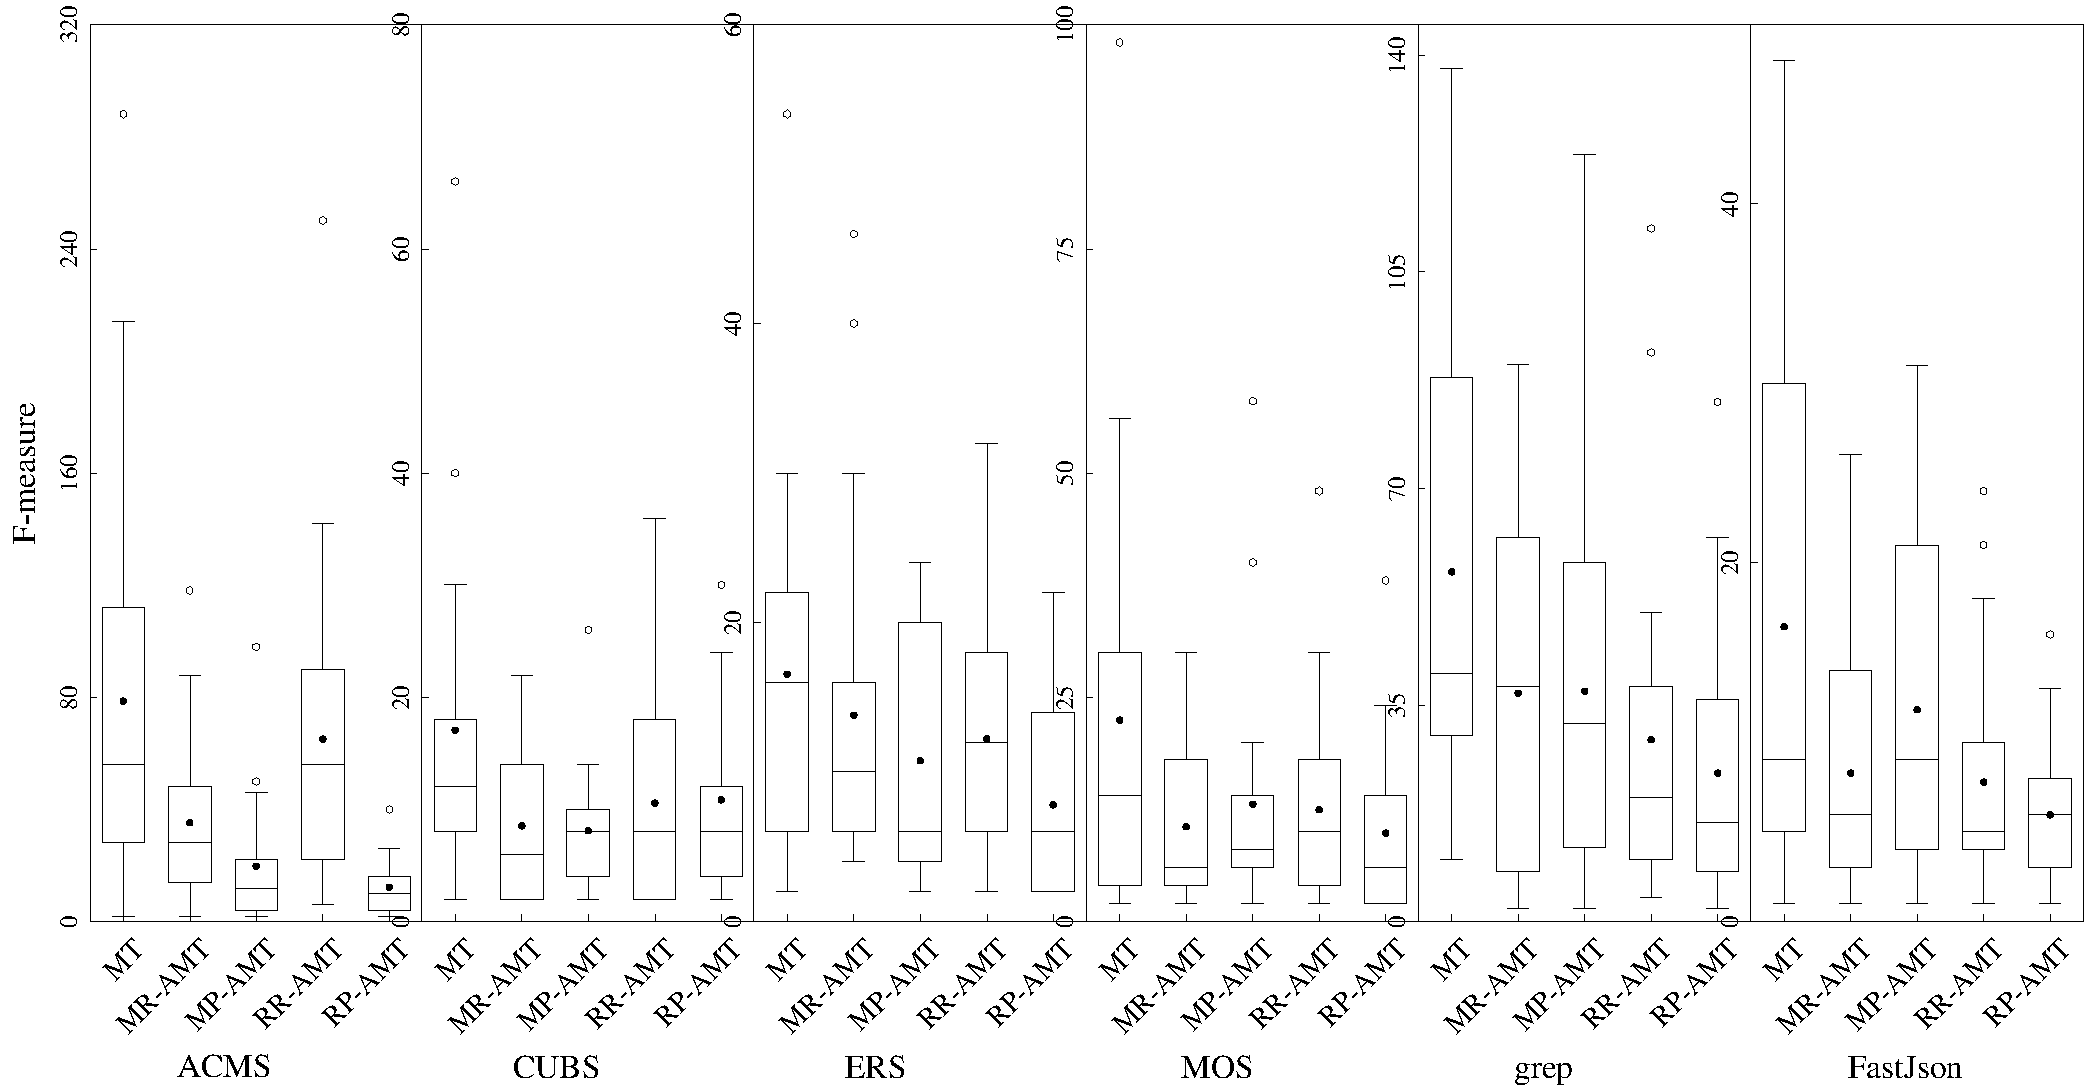
\includegraphics[width = \textwidth,height=6cm]{fig//fmeasure}
  \caption{F-measure boxplots for each program}
  \label{fig:fmeasure}
\end{figure*}

\begin{figure*}[htb]
  \centering
  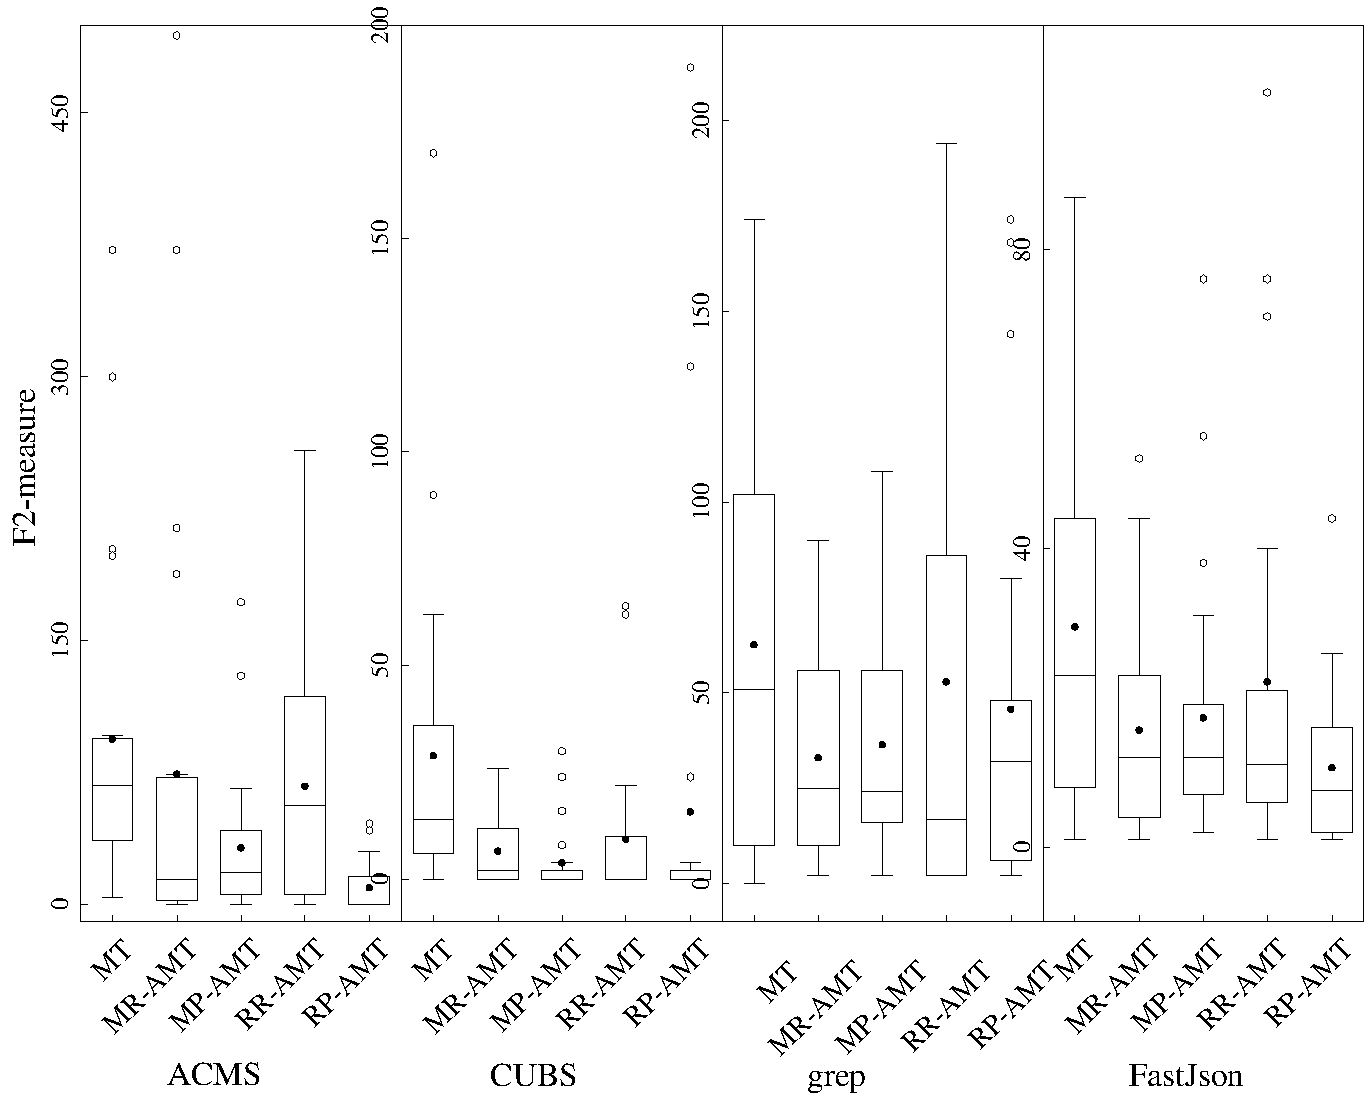
\includegraphics[width = 0.67\textwidth,height=6cm]{fig//f2measure}
  \caption{F2-measure boxplots for each program}
  \label{fig:f2measure}
\end{figure*}



\begin{table}[htbp]
  \caption{Number of Scenarios where the Technique on the top row has a lower metric (F-measure) score than the technique on the left column}
  \centering
  \label{tableHlom:f}
  \renewcommand\tabcolsep{4.0pt}
  \begin{tabular}{llllll}  \toprule
             &MT      &MR-AMT             &MP-AMT             &RR-AMT             &RP-AMT  \\ \midrule
    MT       &---     &\textbf{124}       &\textbf{132}       &\textbf{119}       &\textbf{131}     \\
    MR-AMT   &56      &---                &110                &87                 &107 \\
    MP-AMT   &48      &70                 &---                &92                 &100 \\
    RR-AMT   &61      &93                 &88                 &---                &110 \\
    RP-AMT   &49      &73                 &80                 &70                 &--- \\ \bottomrule
  \end{tabular}
\end{table}

\begin{table}[htbp]
  \caption{Number of Scenarios where the Technique on the top row has a lower metric (F2-measure) score than the technique on the left column}
  \centering
  \label{tableHlom:f2}
  \renewcommand\tabcolsep{4.0pt}
  \begin{tabular}{llllll}  \toprule
             &MT      &MR-AMT             &MP-AMT             &RR-AMT             &RP-AMT  \\ \midrule
    MT       &---     &\textbf{82}       &\textbf{88}         &\textbf{76}        &\textbf{96}     \\
    MR-AMT   &38      &---                &75                 &58                 &85  \\
    MP-AMT   &32      &45                 &---                &61                 &79 \\
    RR-AMT   &44      &62                 &59                 &---                &83 \\
    RP-AMT   &24      &35                 &41                 &37                 &--- \\ \bottomrule
  \end{tabular}
\end{table}

\subsection{RQ2: Selection Overhead}
\label{sec:rq2}

The detailed experimental results of F-time and F2-time are shown in Figures \ref{fig:ftime} and \ref{fig:f2time}. From Figures \ref{fig:ftime} and \ref{fig:f2time}, we can observe that in general, RP-AMT had the best performance, followed by RR-AMT, MR-AMT, and MP-AMT. Note that MR-AMT, MP-AMT, RR-AMT, and RP-AMT do not consistently delivered the best performance for all object programs in terms of both F-time and F2-time, while the larger the program, the better the AMT performs. As we can observe from figure 2, the execution of the test cases accounts for most of the overhead. AMT compensates for the overhead of selecting test cases by reducing the number of test cases executed.

We also conducted hypothesis testing to determine which pair of testing techniques have significant difference in terms of F-time and F2-time, as shown in Tables \ref{tableHlom:ftime} and \ref{tableHlom:f2time}.

From Table \ref{tableHlom:ftime} and \ref{tableHlom:f2time}, we can observe that fourteen entries (``102'' \& ``78'' for MR-AMT versus MT, ``112'' \& ``68'' for MP-AMT versus MT, ``91'' \& ``89'' for RR-AMT versus MT, and ``120'' \& ``60'' for RP-AMT versus MT, ``96'' \& ``84'' for MR-AMT versus MT, ``114'' \& ``66'' for RR-AMT versus MT, and ``128'' \& ``52'' for RP-AMT versus MT) are in bold font. These observations imply that in terms of F-time, AMT performed better than MT (``87'' \& ``93'' for MP-AMT versus MT). On the other hand, the performance of RP-AMT was significantly better than that of the other four techniques. In other words, the additional computation incurred in AMT for updating the probability profiles and selecting MRs is compensated with the saving of test executions.

\begin{figure*}[htbp]
  \centering
    \subfigure[Laboratory programs] {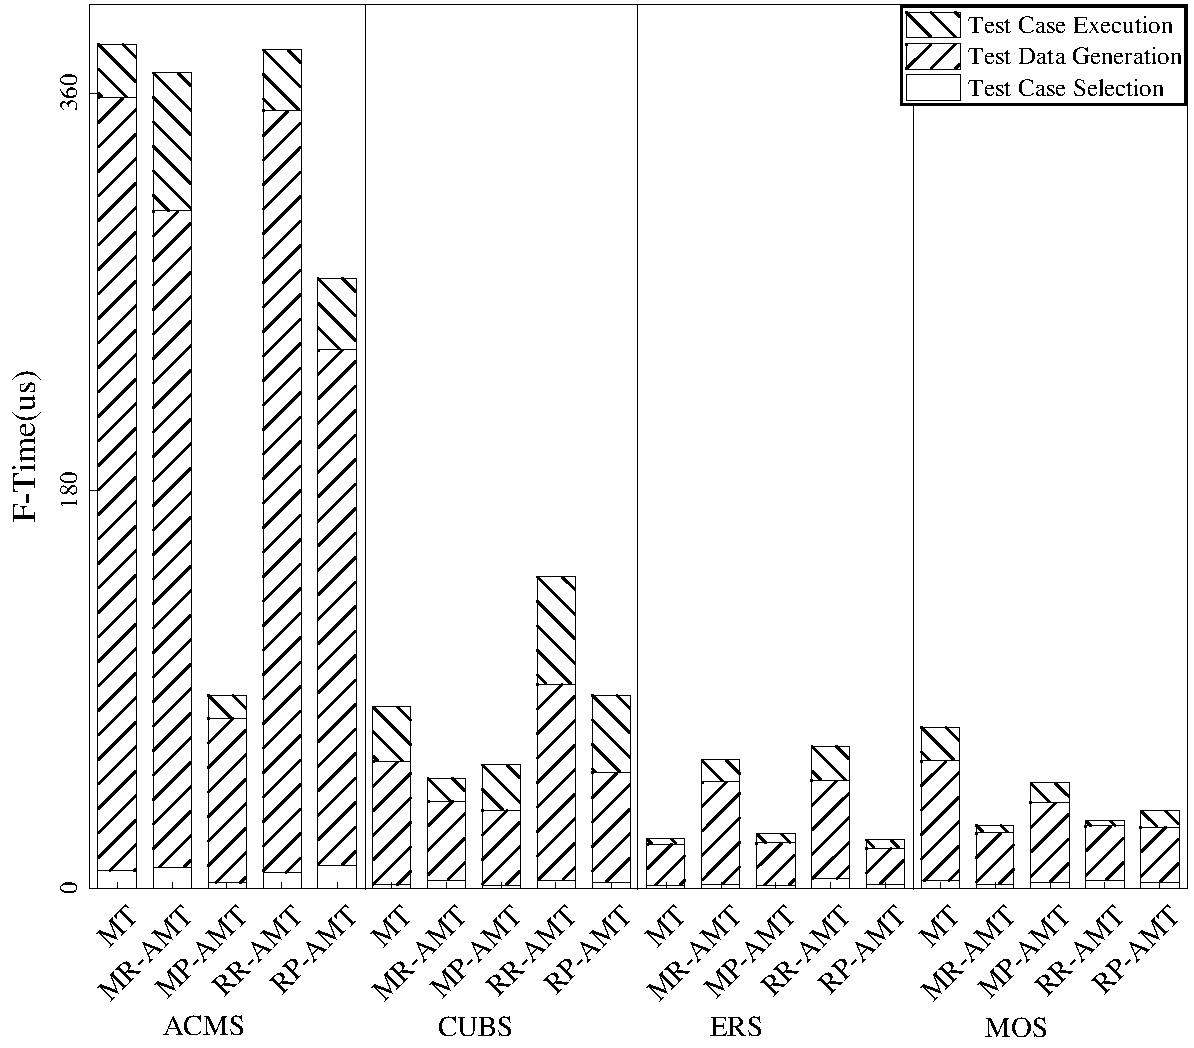
\includegraphics[width=0.49\textwidth,height=5cm]{fig//ftlab}}
    \subfigure[GNU grep] {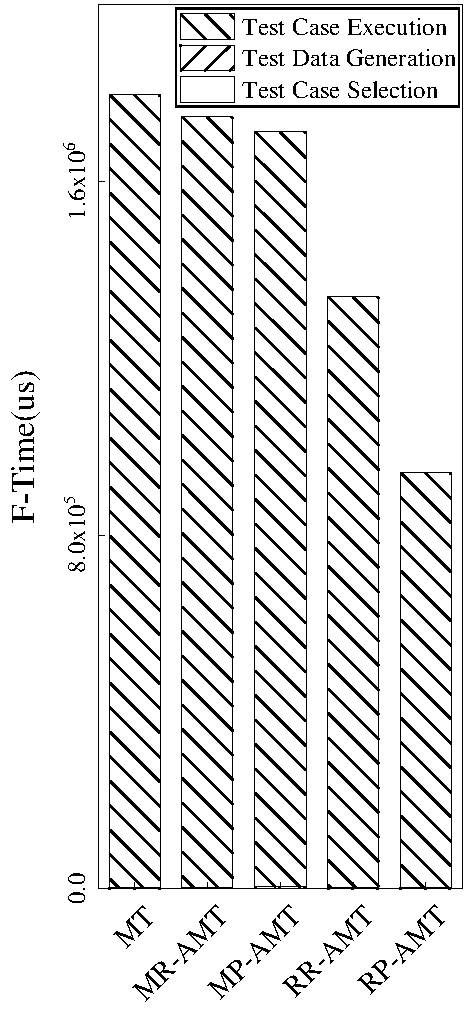
\includegraphics[width=0.23\textwidth,height=5cm]{fig//ftgrep}}
    \subfigure[Alibaba FastJson] {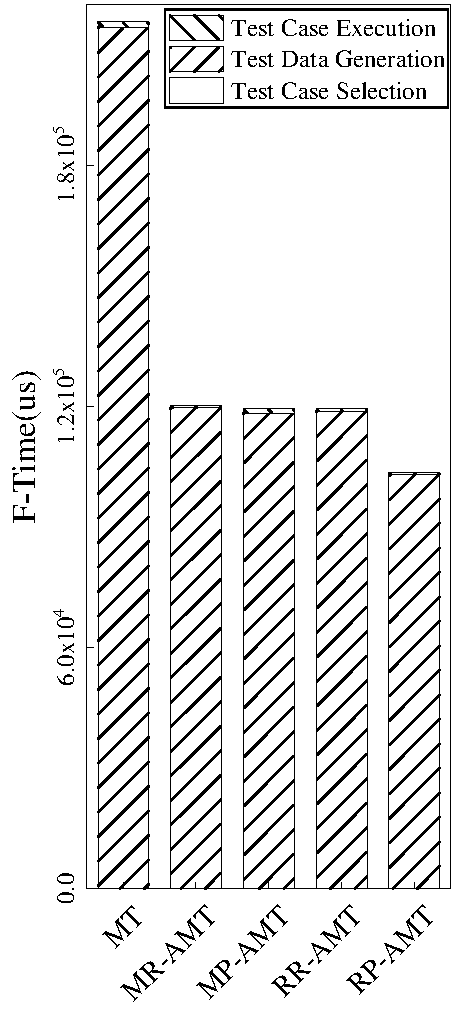
\includegraphics[width=0.23\textwidth,height=5cm]{fig//ftfast}}
  \caption{The F-time results of test case selection, generation, and execution}
  \label{fig:ftime}
\end{figure*}

\begin{figure*}[htbp]
  \centering
    \subfigure[Laboratory programs] {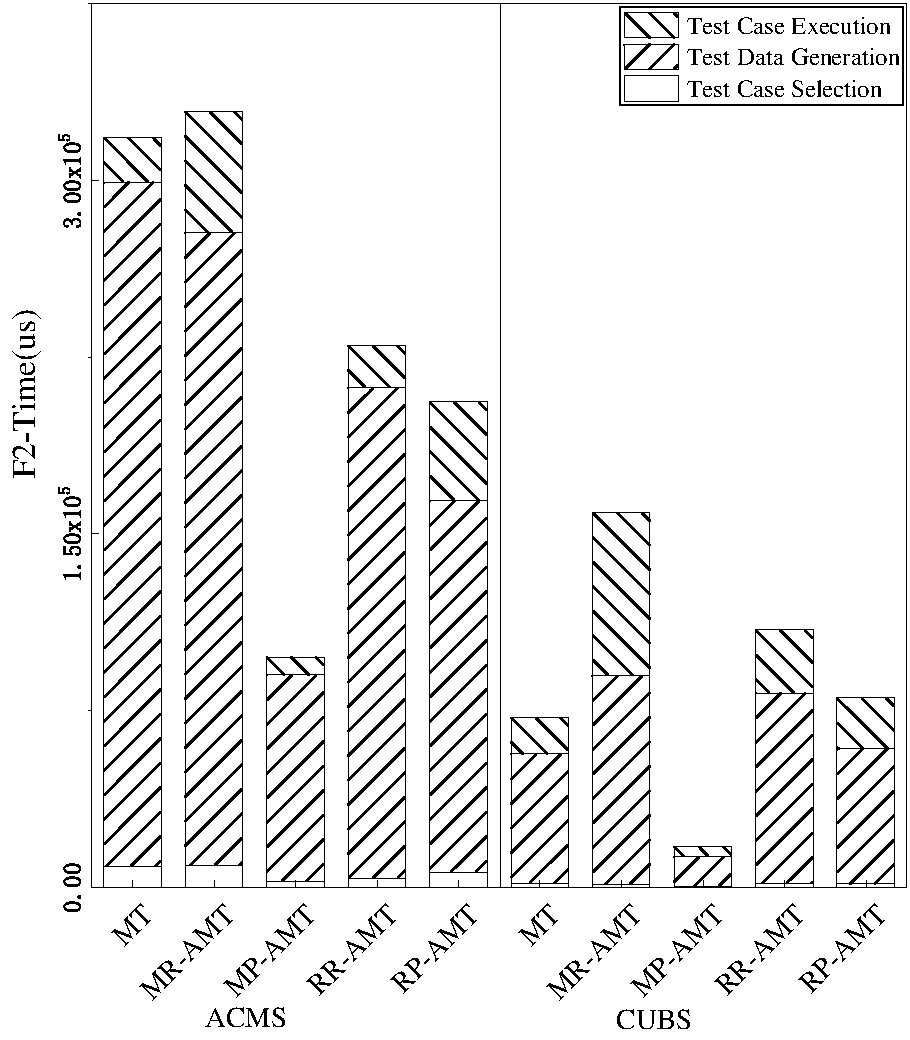
\includegraphics[width=0.49\textwidth,height=5cm]{fig//ft2lab}}
    \subfigure[GNU grep] {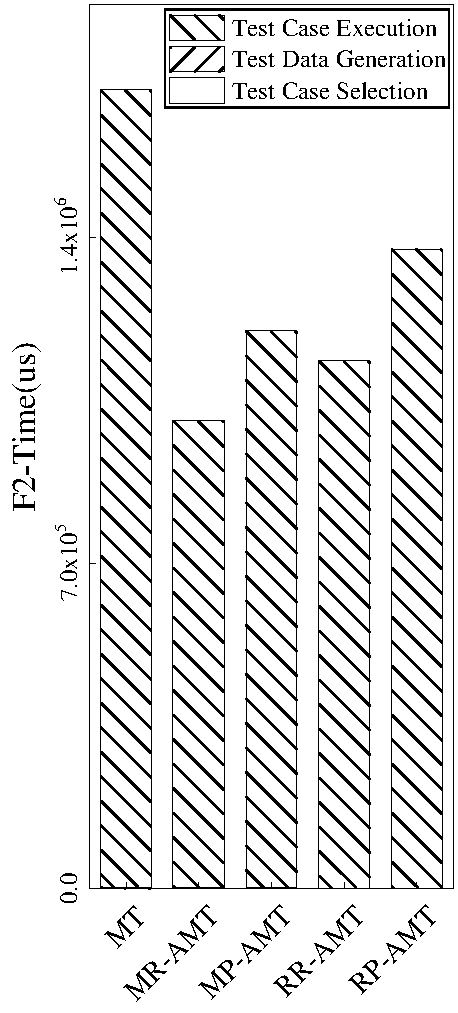
\includegraphics[width=0.23\textwidth,height=5cm]{fig//ft2grep}}
    \subfigure[Alibaba FastJson] {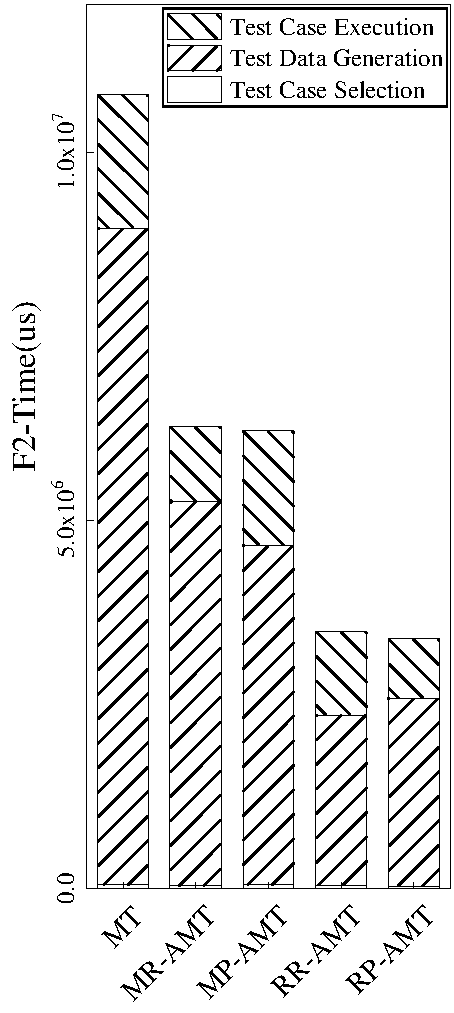
\includegraphics[width=0.23\textwidth,height=5cm]{fig//ft2fast}}
  \caption{The F2-time results of test case selection, generation, and execution}
  \label{fig:f2time}
\end{figure*}


\begin{table}[htbp]
  \caption{Number of Scenarios where the Technique on the top row has a lower metric (F-time) score than the technique on the left column}
  \centering
  \label{tableHlom:ftime}
  \renewcommand\tabcolsep{4.0pt}
  \begin{tabular}{llllll}  \toprule
             &MT               &MR-AMT             &MP-AMT             &RR-AMT             &RP-AMT  \\ \midrule
    MT       &---              &\textbf{102}       &\textbf{112}       &\textbf{91}       &\textbf{120}     \\
    MR-AMT   &\textbf{78}      &---                &98                 &71                 &103 \\
    MP-AMT   &\textbf{68}      &82                 &---                &69                 &97 \\
    RR-AMT   &\textbf{89}      &109                &111                &---                &113 \\
    RP-AMT   &\textbf{60}      &77                 &83                 &67                 &--- \\ \bottomrule
  \end{tabular}
\end{table}

\begin{table}[htbp]
  \caption{Number of Scenarios where the Technique on the top row has a lower metric (F2-time) score than the technique on the left column}
  \centering
  \label{tableHlom:f2time}
  \renewcommand\tabcolsep{4.0pt}
  \begin{tabular}{llllll}  \toprule
             &MT              &MR-AMT             &MP-AMT             &RR-AMT             &RP-AMT  \\ \midrule
    MT       &---             &\textbf{66}        &84                 &\textbf{83}        &\textbf{84}     \\
    MR-AMT   &\textbf{54}     &---                &74                 &59                 &73  \\
    MP-AMT   &\textbf{36}     &46                 &---                &47                 &49 \\
    RR-AMT   &\textbf{37}     &61                 &73                 &---                &67 \\
    RP-AMT   &\textbf{36}     &47                 &71                 &53                 &--- \\ \bottomrule
  \end{tabular}
\end{table}

\subsection{Threats To Validity}

\subsubsection{Internal Validity}
A threat to internal validity is related to the implementations of the testing techniques, which involved a moderate
amount of programming work. However, our code was cross-checked by different individuals, and we are confident that all techniques were correctly implemented.

\subsubsection{External Validity}
The possible threat to external validity is related to the subject programs and seeded faults under evaluation. Although
the four laboratory programs are not very complex, they do implement real-life business scenarios of diverse application
domains. Furthermore, we chose two open source programs (\texttt{grep and FastJson}). Although we have tried to improve the generalisability of the findings by applying subject programs in different areas, we anticipate that the evaluation results may vary slightly with different subject web services.

\subsubsection{Construct Validity}
The metrics used in our study are simple in concept and straightforward to apply, and hence there should be little
threat to the construct validity.

\subsubsection{Conclusion Validity}
As reported for empirical studies in the field of software engineering \cite{arcuri2011practical}, at least 30 observations are necessary to ensure the statistical significance of results. Accordingly, we have run a sufficient number of trials to ensure the
reliability of our experimental results. Furthermore, as will be discussed in Section 5, we also conducted statistical tests
to confirm the significance of the results.

\section{Related Work}
\label{sec:relatedwork}

When testing a software system, the oracle problem appears in some situations where either an oracle does not exist for the tester to verify the correctness of the computed results; or an oracle does exist but cannot be used. The oracle problem often occurs in software testing, which renders many testing techniques inapplicable \cite{barr2015oracle}. To alleviate the oracle problem, Chen et al. \cite{chen1998metamorphic} proposed a technique named metamorphic testing (MT) that has been receiving increasing attention in the software testing community\cite{barr2015oracle, segura2016survey, chen2018metamorphic}. To improve the fault-detecting efficiency of MT, researchers mainly focus on the following aspects: \rmnum{1}) MR; \rmnum{2}) source test case.

The MRs and the source test cases are the most important components of MT. However, defining MRs can be difficult. 
Chen et al. \cite{chen2016metric} proposed a specification-based method and developed a tool called MR-GENerator for identifying MRs based on category-choice framework\cite{ostrand1988category}.
Zhang et al. \cite{zhang2014search} proposed a search-based approach to automatic inference of polynomial MRs for a software under test, where a set of parameters is used to represent polynomial MRs, and the problem of inferring MRs is turn into a problem of searching for suitable values of the parameters. Then, particle swarm optimization is used to solve the search problem.
Sun et al. \cite{sun2016mumt} proposes a data-mutation directed metamorphic relation acquisition methodology, in which data mutation is employed to construct input relations and the generic mapping rule associated with each mutation operator to construct output relations.
Liu et al. \cite{liu2012new} proposed to systematically construct MRs based on some already identified MRs.

With the development of various identification MR methods, how to select efficient MR from a large number of MR has become an urgent problem to be solved.
Chen et al. \cite{chen2004metamorphic} initially suggested all available metamorphic relations, of which each one might have sensitivity to different faults, should be used as part of the test strategy. 
However, the resources for software development are always limited. 
Chen et al. \cite{chen2004case} proposed good MRs should be those that can make the multiple executions of the program as different as possible. Furthermore, they proposed that good MRs should be selected with regard to the algorithm that the program follows. 
However, Mayer et al. confirmed the usefulness of whitebox considerations proposed in \cite{chen2004case} and refined the informal criterion (``different execution path'') to criteria underlying or used in the implementation/algorithm. Asrafi et al. \cite{asrafi2011testing} conducted a case study to analyze the relationship between the execution behavior and the fault-detection effectiveness of metamorphic relations, and some code coverage criteria are used to reflect the execution behavior. It is shown that the higher the combined code coverage of the source and follow-up test cases, the more different are the executions, and the more effective is the metamorphic relation. 
Just et al. \cite{Just2010Automating} assessed the applicability of metamorphic testing for system and integration testing in the context of an image encoder, and concluded that the metamorphic relations derived from the components of a system are usually better at detecting faults than those metamorphic relations derived from the whole system. This finding was later confirmed by Xie et al. \cite{xie2014bottom}. 

The existing metamorphic relationship selection strategies require the execution of test cases for MR selection, which increases the resource overhead of software testing. Since AMT selects efficient MRs through analyzing historical information in the testing process, it saves testing resources.

Source test cases also have a important impact on the fault detection efficiency of MT. However, 57\% of existing studies employed RT to select test cases, and 34\% of existing studies used existing test suites according to a survey report by Segura et al. \cite{segura2016survey}. In other words, investigation of the impact of source test cases on MR (and MT) effectiveness and efficiency are an area yet to be explored. 
Chen et al. \cite{chen2004metamorphic} compared the effects of source test cases generated by special value testing and random testing on the effectiveness of MT, and found that MT can be used as a complementary test method to special value testing.
Batra and  Sengupta \cite{batra2011efficient} integrated genetic algorithms into MT to select source test cases maximising the the paths traversed in the software under test.
Dong et al. \cite{dong2013security} proposed a Path--Combination--Based MT method that first generates symbolic input for each executable paths and minis relationships among these symbolic inputs and their outputs, then constructs MRs on the basis of these relationships, and generates actual test cases corresponding to the symbolic inputs.
Barus et al. \cite{barus2016impact} employed adaptive random testing \cite{chen2004adaptive} that is a class of testing method aimed to improve the performance of RT by increasing the diversity across a program's input domain of the test cases executed to generate source test cases for MT.

Different from the above investigates, we focused on performing test cases and MRs with fault revealing capabilities as quickly as possible by making use of feedback information. We first divided the input domain into disjoint partitions, and randomly selected an MR to generate follow-up test cases depended on source test case of related input partitions, then updated the test profile of input partitions according to the results of test execution. Next, a partition was selected according to updated test profile, and an MR was randomly selected from the set of MRs whose source test cases belong to selected partition.

\section{Conclusion}
\label{sec:conclusion}
In this paper, to improve the efficiency of MT, we have presented an adaptive metamorphich testing framework, and proposed two source test case selection strategies and two MRs selection strategies based on software cybernetics. Our method makes use of the historical information of the test to dynamically select the source test cases and MRs with higher fault-detecting ability during the test process.

In the proposed AMT framework, there is a feedback loop, which constitutes the components of MT, the software under
test, the history of testing data and the testing strategy, where the testing history is uesed to select the next source test case and MR. Besides, The source test case selection strategy and MR selection strategy are updated during the test process by changing the values of parameters of source test case selection strategy and MR selection strategy. Six subject programs (including four laboratory programs, a GNU program, and an Alibaba program) were used as experimental subjects to validate the feasibility and efficiency of our approach. Our experimental results show that, AMT has better performance than MT, in terms of the F-measure, F2-measure, F-time, and F2-time.

In our future work, we plan to proposed new source test case and MR selection strategies based on AMT framework, and identify the limitations of our method. 


\section*{Acknowledgment}

This research is supported by
the National Natural Science Foundation of China (Grant No. 61872039),
the Beijing Natural Science Foundation (Grant No. 4162040),
the Aeronautical Science Foundation of China (Grant No. 2016ZD74004), and
the Fundamental Research Funds for the Central Universities (Grant No. FRF-GF-19-B19).
\ifCLASSOPTIONcaptionsoff
  \newpage
\fi
\bibliographystyle{IEEEtran}
\bibliography{AMT}
\begin{IEEEbiography}[{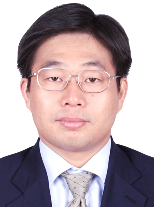
\includegraphics[width=1in,height=1.25in,clip,keepaspectratio]{fig/authors/CASun.pdf}}]{Chang-ai Sun} is a Professor in the School of Computer and Communication Engineering, University of Science and Technology Beijing.
Before that, he was an Assistant Professor at Beijing Jiaotong University, China, a postdoctoral fellow at the Swinburne University of Technology, Australia, and a postdoctoral fellow at the University of Groningen, The Netherlands. He received the bachelor degree in Computer Science from the University of Science and Technology Beijing, China, and the PhD degree in Computer Science from Beihang University, China.
His research interests include software testing, program analysis, and Service-Oriented Computing.
\end{IEEEbiography}
\begin{IEEEbiography}[{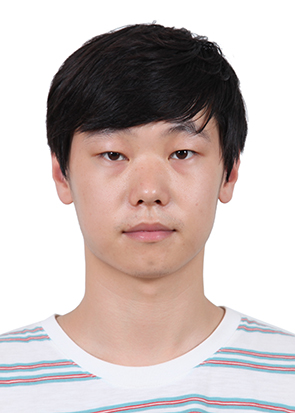
\includegraphics[width=1in,height=1.25in,clip,keepaspectratio]{fig/authors/HPDai.jpg}}]{Hepeng Dai} is a PhD student in the School of Computer and Communication Engineering, University of Science and Technology Beijing, China. He received the master degree in Software Engineering from University of Science and Technology Beijing, China and the bachelor degree in Information and Computing Sciences from China University of Mining and Technology, China. His current research interests include software testing and debugging.
\end{IEEEbiography}
\begin{IEEEbiography}[{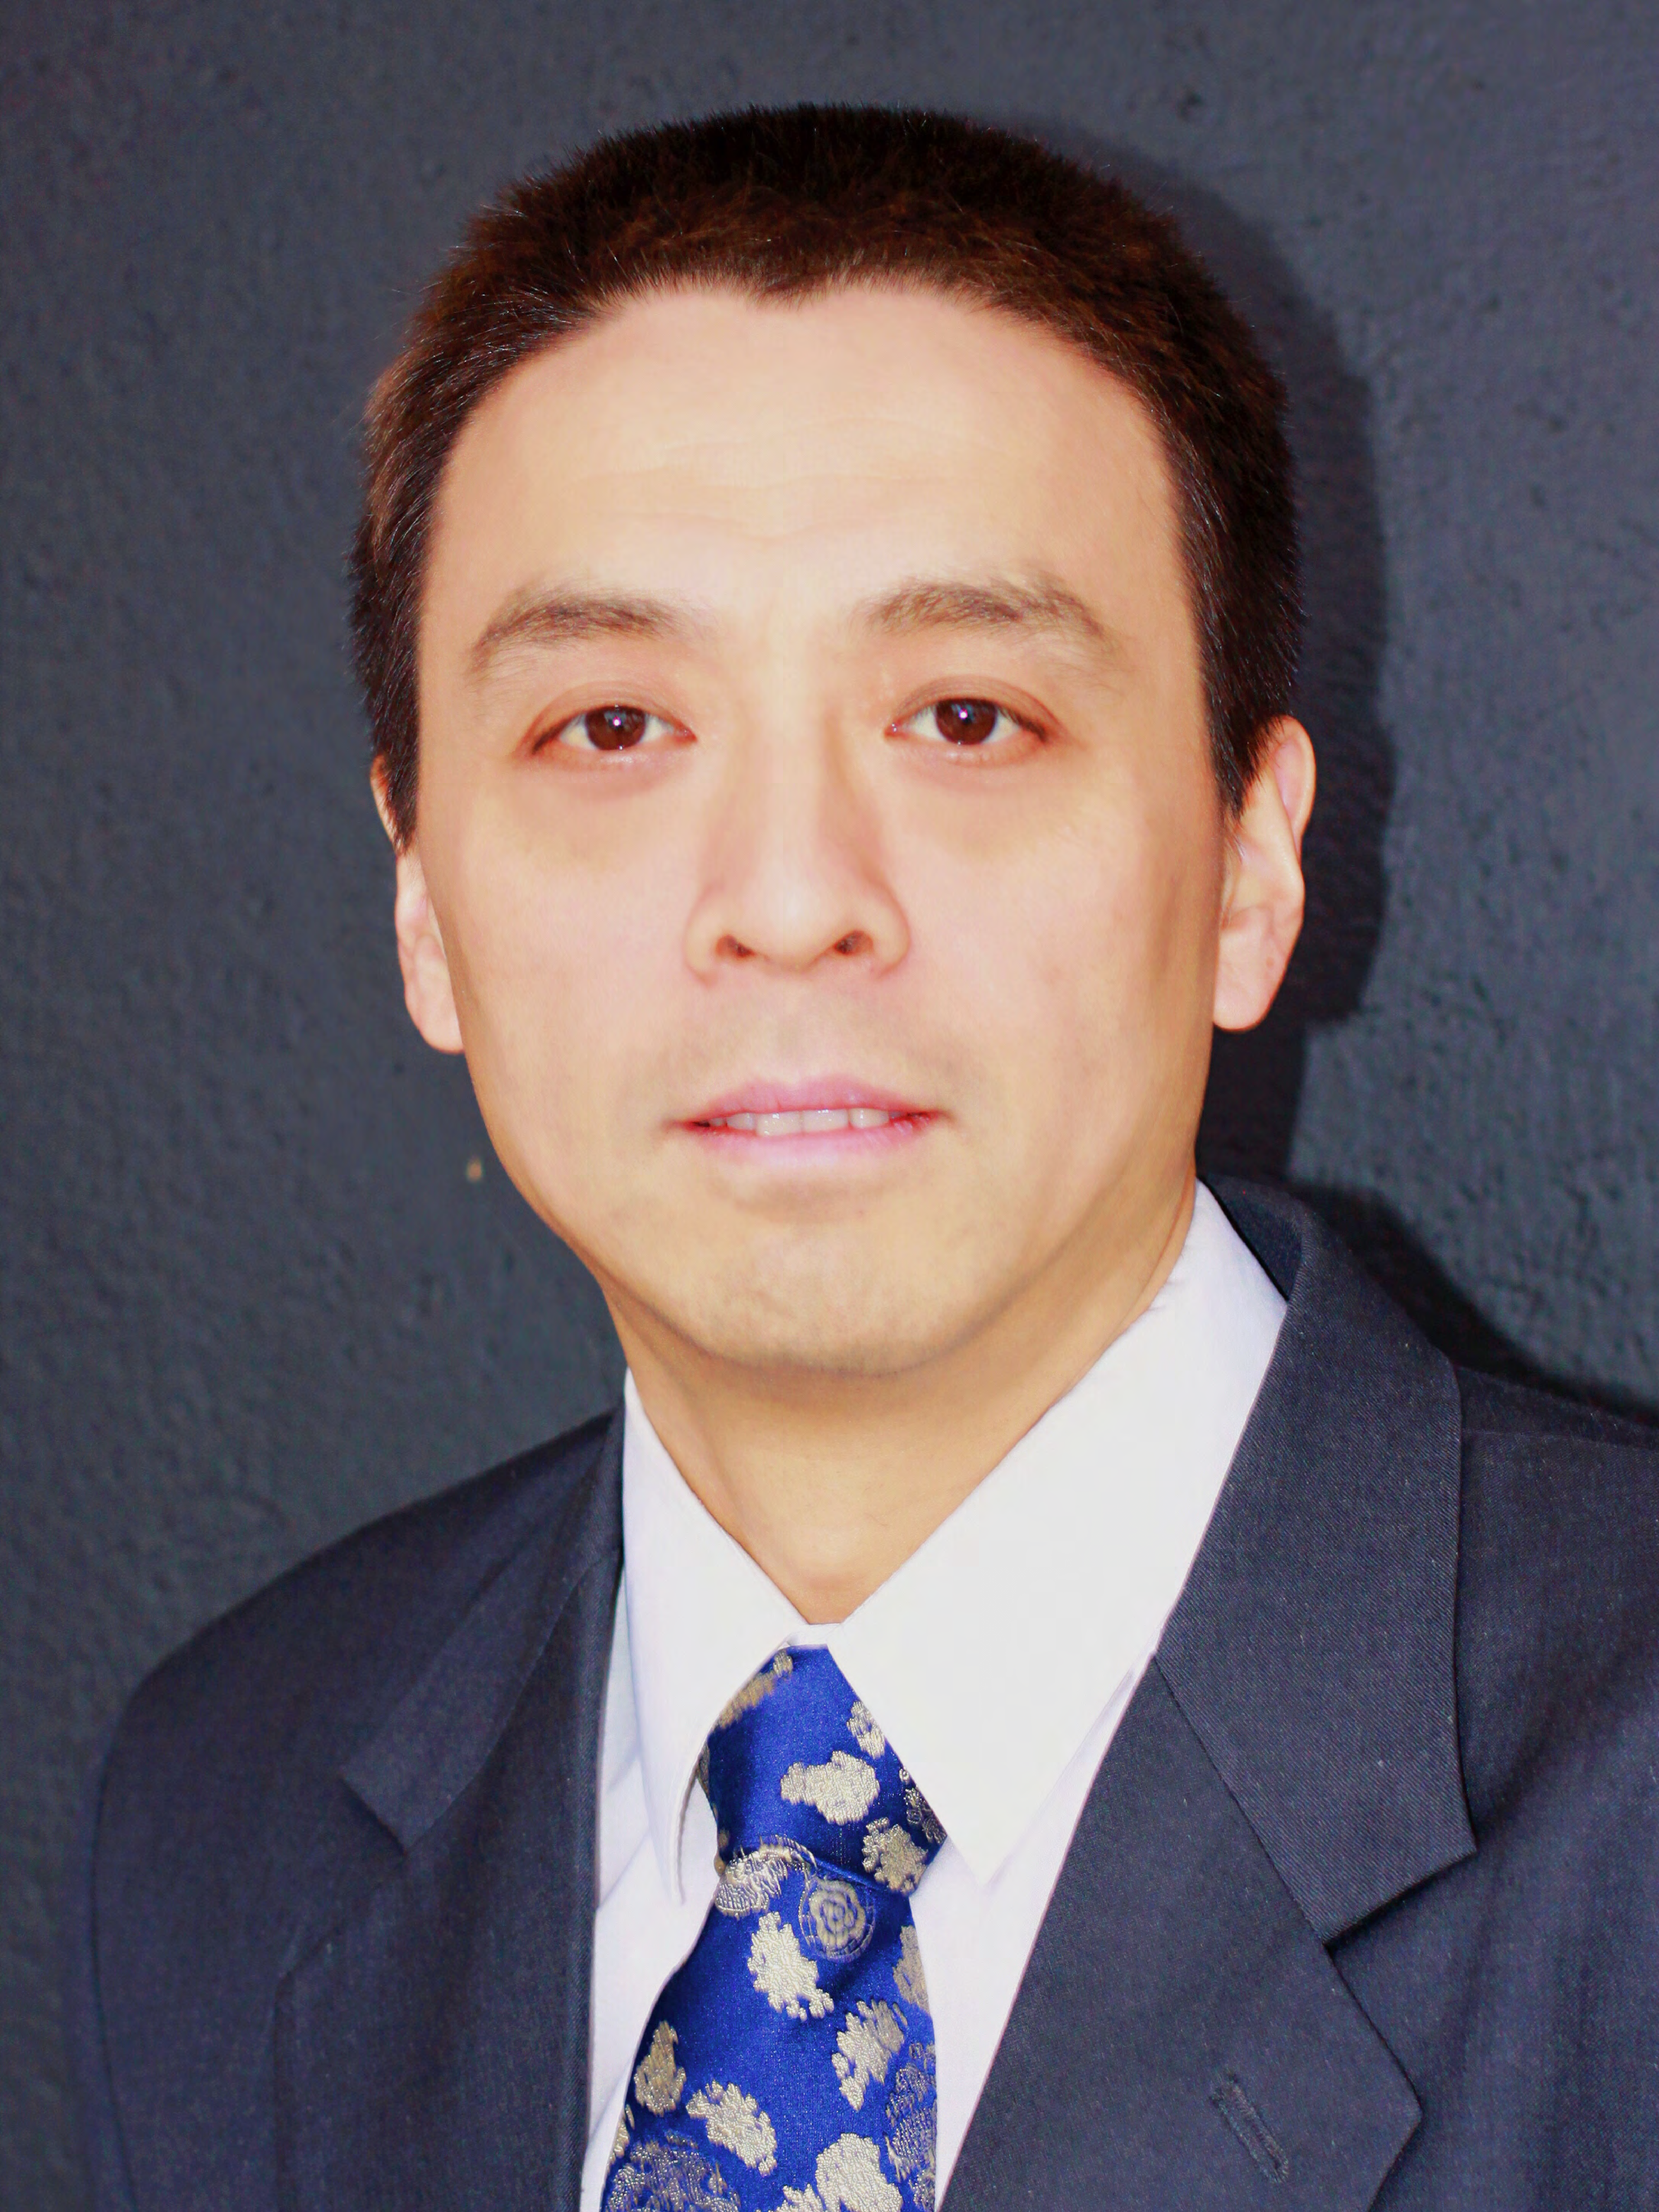
\includegraphics[width=1in,height=1.25in,clip,keepaspectratio]{fig/authors/HLiu.pdf}}]{Huai Liu} is a Lecturer of Information Technology at the College of Engineering \& Science in Victoria University, Melbourne, Australia. Prior to joining VU, he worked as a research fellow at RMIT University and a research associate at Swinburne University of Technology. He received the BEng in physioelectronic technology and MEng in communications and information systems, both from Nankai University, China, and the PhD degree in software engineering from the Swinburne University of Technology, Australia. His current research interests include software testing, cloud computing, and end-user software engineering.
\end{IEEEbiography}
\begin{IEEEbiography}[{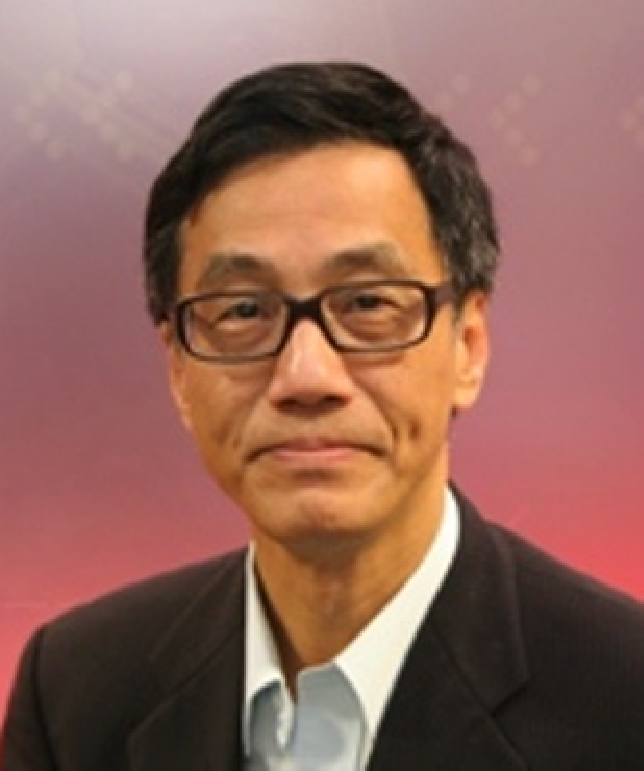
\includegraphics[width=1in,height=1.25in,clip,keepaspectratio]{fig/authors/TYChen.pdf}}]{Tsong Yueh Chen} is a Professor of Software Engineering at the Department of Computer Science and Software Engineering in Swinburne University of Technology. He received his PhD in Computer Science from The University of Melbourne, the MSc and DIC from Imperial College of Science and Technology, and BSc and MPhil from The University of Hong Kong. He is the inventor of metamorphic testing and adaptive random testing.
\end{IEEEbiography}


\end{document}
